\documentclass[t,usenames,dvipsnames]{beamer} % [t] pomeni poravnavo na vrh slida

    % \State Randomly choose rewriting rule 
    % \State choose rewriting rule Randomly 
    % relation closure more verbose on slides

% \usepackage{etex} % vključi ta paket, če ti javi napako, da imaš naloženih preveč paketov.
% \usefonttheme[stillsansserifsmall,stillsansseriflarge]{serif}

% \usepackage{amsfonts}
% \usepackage[mathscr]{eucal}
% \usepackage[mathscr]
\usepackage{mathrsfs}


% standardni paketi
\usepackage[slovene]{babel}
\usepackage[T1]{fontenc}
\usepackage[utf8]{inputenc}
\usepackage{amsmath,amssymb,amsfonts,amsthm} % matematični paketi
% \usepackage{amssymb}
% \usepackage{amsmath}
% \usepackage{diagrams}
\usepackage{array}
\usepackage{multirow}
\usepackage{qtree}
	\usepackage{forest}
\forestset{
dg edges/.style={for tree={parent anchor=south, child anchor=north,align=center,base=bottom,where n children=0{tier=word,edge=dotted,calign with current edge}{}}},
dgii edges/.style={for tree={parent anchor=south, child anchor=north,base=bottom}},
}

\newcommand{\pgrammar}{
    R :  \\
    S $\to$ Subject Verb Object [0.3] \\
    S $\to$ Subject Verb Object Manner [0.7] \\
    Manner $\to$ with Object [1] \\
    Verb $\to$ see [0.9] \\
    Verb $\to$ invent [0.1] \\
    Subject $\to$ Subject with Subject [0.2] \\
    Subject $\to$ dog [0.3] \\
    Subject $\to$ telescope [0.5]
}

% \newcommand{\grammar}{
%       \only<2>{R :=  \\
%     S $\to$ Povedek Predmet \\
%     S $\to$ Povedek Predmet Prislovno\_dolocilo\_nacina [0.7] \\
%     Prislovno\_dolocilo\_nacina $\to$ s Predmet [1] \\
%     Povedek $\to$ vidim [0.9] \\
%     Povedek $\to$ dokazujem [0.1] \\
%     Predmet $\to$ Predmet s Predmet [0.2] \\
%     Predmet $\to$ psa [0.3] \\
%     Predmet $\to$ teleskopom [0.5]} 
% }

\usepackage{fp}
% \newcommand{\add}[2]{ \FPeval{ \p }{round(#1+#2, 0)} \p }
\newcommand{\eval}[1]{ \FPeval{ \p }{round(#1, 0)} \p }
% \newcommand{\add}[2]{ \FPeval{ \p }{#2+#1} \p }
% \newcommand{\add}[2][2]{ \FPeval{ \p }{round(#2, #1)} \p }
% \newcommand{\datan}[1]{
% \newcommand{\datatwo}[1]{
%     \( \left[ \begin{array}{ccccccccc}
%         a_1 & a_2 &  a_{\eval{#1+1}} \\
%         a_2 & a_3 &  a_{\eval{#1+2}} \\
%     \vdots & \vdots  & \vdots \\
%         a_{\eval{50-#1}} & a_{\eval{50-(#1-1)}} & a_{50} \\
%     \end{array} \right] \)}
% \newcommand{\dataset}[1]{
%     \( \left[ \begin{array}{ccccccccc}
%         a_1 & a_2 & \cdots & a_{\eval{#1+1}} \\
%         a_2 & a_3 & \cdots & a_{\eval{#1+2}} \\
%     \vdots & \vdots & \ddots & \vdots \\
%         a_{\eval{50-#1}} & a_{\eval{50-(#1-1)}} & \cdots & a_{50} \\
%     \end{array} \right] \)}
% \newcommand{\datatwon}[1]{
%     \( \left[ \begin{array}{ccccccccc}
%         1 & a_1 & a_2 &  a_{\eval{#1+1}} \\
%         2 & a_2 & a_3 &  a_{\eval{#1+2}} \\
%     \vdots & \vdots & \vdots  & \vdots \\
%         \eval{50-#1} & a_{\eval{50-#1}} & a_{\eval{50-(#1-1)}} & a_{50} \\
%     \end{array} \right] \)}
% \newcommand{\datasetn}[1]{
%     \( \left[ \begin{array}{ccccccccc}
%         1 & a_1 & a_2 & \cdots & a_{\eval{#1+1}} \\
%         2 & a_2 & a_3 & \cdots & a_{\eval{#1+2}} \\
%     \vdots & \vdots & \vdots & \ddots & \vdots \\
%        \eval{50-#1} & a_{\eval{50-#1}} & a_{\eval{50-(#1-1)}} & \cdots & a_{50} \\
%     \end{array} \right] \)}


\newcommand{\algoii}{
    \begin{algorithm}[H]
    \caption{Function \textit{generate}, that uses probabilistic grammars
        % ki uporablja verjetnostne % kontekstno-neodvisne gramatike}
        }
    % \label{algo:create}
    \raggedright
    \textbf{Input:} Probabilistic grammar $G=(N,T,R,S)$, 
    % nekon"cni 
        symbol $A \in N$ \\
    \textbf{Output:} Sentence $s$ in grammar $G$
    %   Seznam $ena"cbe$, ki vsebuje pare ena"cb in njihovih napak.
    \begin{algorithmic}[1]
    \Function{Generate}{$G$, $A$} %\Comment{Vsi vhodni parametri morajo biti opisani.}
    \State $s \gets [\,\,]$ 
    % \State Izberi naključno pravilo 
    \State Randomly choose rewriting rule 
    $(A \to A_1\ A_2 \cdots A_k ) \in R$
    % , kjer $\alpha = $
    \For{$i=1, ..., k$}
    \If{$A_i \in T$} 
    \State $s = s$.append($A_i$) 
    \Else 
    \State $s_i$ = \Call{Generate}{$G$, $A_i$}
    \State $s = s$.append($s_i$) 
    \EndIf
    \EndFor
    % \label{algo:pomembna-vrstica}
    \State \Return $s$
    \EndFunction
    \end{algorithmic}
    \end{algorithm}
}


\DeclareMathOperator{\Coverage}{Coverage} 

% % down 4.4.2017
\newcommand{\R}{\mathbb R}
% \newcommand{\N}{\mathbb N}
% \newcommand{\Z}{\mathbb Z}
\newcommand{\C}{\mathbb C}
\newcommand{\Q}{\mathbb Q}
\definecolor{softyellow}{rgb}{0.98,0.98,0.75}
\setbeamercolor{loweryel}{fg=black,bg=softyellow}
% % up 4.4.2017
\newcommand{\e}{\boldsymbol{e}}
\newcommand{\X}{\mathscr{X}}
\newcommand{\I}{\mathscr{I}}
\newcommand{\rhoo}{\boldsymbol{\rho}}
\newcommand{\q}{\boldsymbol{q}}
\newcommand{\1}{\boldsymbol{1}}
\newcommand{\0}{\boldsymbol{0}}
\newcommand{\N}{\mathbb{N}}
\newcommand{\Nom}{\mathbb{N}_0^m}
\newcommand{\Z}{\boldsymbol{Z}}
\newcommand{\Zn}{\boldsymbol{Z}_n}
\newcommand{\M}{\boldsymbol{M}}
\newcommand{\re}{\boldsymbol{r}}
% \newcommand{\r}{\boldsymbol{r}}
\renewcommand{\r}{\boldsymbol{r}}
\newcommand{\s}{\boldsymbol{s}}
% glej $$ \r $$ 
% \newcommand{\e}{\boldsymbol{e}}
\renewcommand{\e}{\boldsymbol{e}}

% \newtheorem{lemma}{Lemma}
% \newtheorem{definition}{Definition}
% \newtheorem{theorem}{Theorem}



%\setbeamercovered{invisible} %default
\setbeamercovered{transparent}
%\setbeamercovered{dynamic}


%\usepackage[dvipsnames]{color}

\usepackage[normalem]{ulem} % za strikeout (prečrtat besedo)
% na primer : \sout{Hello World}

% podatki
\title{Equation discovery for integer sequences with probabilistic grammars}
\author{Boštjan Gec}
\institute{mentor: prof. dr. Ljupčo Todorovski}

% tvoj izbran stil predstavitve
%\usetheme{Singapore}
\usetheme{Luebeck}
%\usecolortheme{crane}
%\usecolortheme{red}

\usepackage{color}
\setbeamercolor{structure}{fg=Bittersweet}
\setbeamercolor{structure}{fg=ForestGreen}


% \usepackage{algorithmic}
\usepackage{algpseudocode}  % za psevdokodo
\usepackage{algorithm}
% \floatname{algorithm}{Algoritem}
% \renewcommand{\listalgorithmname}{Kazalo algoritmov}
\usepackage{multirow}

\usepackage{hyperref}

\begin{document}


\begin{frame}
  \maketitle
%  \fillblack{0.33}
\end{frame}


% \section{Equation discovery}
% \section{Verjetnostne gramatike}
% \section{Celo"stevilska zaporedja}

\begin{frame}{Introduction}
\begin{block}{Equation discovery for integer sequences with probabilistic grammars}
\begin{itemize}
	\item Equation discovery
	\item Probabilistic grammars
	\item Integer sequences
\end{itemize}
\end{block}
\end{frame}

\section{Equation discovery}

% \begin{frame}{Algoritem za odkrivanje ena"cb}
% \frametitle{Naslov prosojnice}
% \framesubtitle{Linearna regresija}
% % 	\begin{block}{Odkrivanje enačb za celoštevilska zaporedja z verjetnostnimi gramatikami}
% % \pause
% % \invisible<1>{Trije koraki:}
% Trije koraki:
% \pause
% \begin{enumerate}
% % [<+->]
% 	\item Struktura ena"cbe \(y = c_0 + c_1\cdot x_{1}  +
% 	c_2\cdot x_{2}+ \cdots + c_n\cdot x_{n}  \)
% \item Napaka modela \[ \sum_{i=1} ^m (y _i - c_0 + c_1\cdot x_{i1}  +
% 	c_2\cdot x_{i2}+ \cdots + c_n\cdot x_{in} )^2
% 	\]
% kjer je $n+1$ "stevilo stolpcev, m "stevilo vrstic, $y_i$ element matrike X v i-ti vrstici
% in $(n+1)$-tem stolpcu, $x_{ij}$ element matrike X v i-ti vrstici in j-tem stolpcu.\\
% 	X = [x|y]
% 	\item Optimizacija konstant \( c_0, c_1, ..., c_n \), da bo
% 	napaka modela "cim manj"sa.
% \end{enumerate}

% \end{frame}

\begin{frame}{Algorithm for equation discovery}
\framesubtitle{Dataset}
% \begin{enumerate}[<+->]
%         \item Podatkovna mno"zica
% \end{enumerate}

    \only<1>{
\textbf{Dataset} is a matrix
\( X \in \mathbb{R}^{m \times n} \), 
where:
\begin{itemize}
    \item columns correspond to \textbf{observed (numeric) variables (features)}, that we usually  \(x_1, x_2, ..., x_n\) ter
\item rows correspond to \textbf{instances} and each instance is made up of measured values of observed variables.
\end{itemize}

    Therefore:
	\[ X = 
     \left[ \begin{array}{ccccc}
         x_{11} & x_{12} & \cdots &  x_{1n}  \\
         x_{21} & x_{22} & \cdots &  x_{2n}  \\
        \vdots  &  & \ddots &  \vdots  \\
         x_{m1} & x_{m2} & \cdots &  x_{mn}  \\
	\end{array} \right] 
    = \left[ \begin{array}{ccccc}
		x_1 & x_2 & \cdots & x_n \\
	\end{array} \right] \]

}

\pause

For example:
\begin{table}[h]
\centering
\begin{center}
\(
% \label{tab:ptv}
\begin{array}{ccc}
% \text{Tlak ($p$ oz. $y$) [$kPa$]  } & 
% \text{Temperatura ($T$ oz. $x_1$) [ \SI{}{\degreeCelsius} ]   } &
% \text{Prostornina ($V$ oz. $x_2$) [$l$] } \\
\hline
\text{Temperature ($x_1$) [% \SI{}{\degreeCelsius} 
\textrm{K}]   } &
\text{Volume ($x_2$) [\textrm{l}] } & \text{Pressure ($x_3$) [$\textrm{kPa}$]  } \\

\hline
291 & 6.97 & 348.26 \\
285 & 9.12 & 260.24 \\
% 313 & 7.45 & 350.30 \\
\vdots & \vdots & \vdots \\
307 & 6.61 & 386.84 \\
\hline
\end{array} 
\)
% \caption{podatkovna mno"zica eksperimenta}
\end{center}
\caption{Table of measurements of physical experiment.}
\label{tab:plinska.enacba}
\end{table}

This way we get dataset $X$ of dimension \(50\times 3\).
% Na ta na"cin smo dobili podatkovno mno"zico X dimenzij \(50\times 3\).


\end{frame}


\begin{frame}{Algorithm for equation discovery}
% \begin{frame}{Algoritem za odkrivanje ena"cb}
\framesubtitle{Task of equation discovery}
% \framesubtitle{Naloga odkrivanja ena"cb}
% Podobni trije koraki:
% \begin{enumerate}[<+->]
\begin{itemize}[<+->]
% \item Generira seznam struktur izrazov (za ena"cbe). 
% 	Struktura ena"cba \(y = \textcolor{red}{izraz}(c_0, \cdots,  c_k, x_{1}, \cdots, x_{n}) \) 
    \item The task is to find out equations of the form:
    % \item Naloga je poiskati ena"cbe oblike:
       % \begin{equation}
            $$
            x_n = f(\vec{c}, \vec{x}) \uncover<2>{ = f((c_1, ..., c_k), (x_1, x_2, ..., x_{n-1})) }  \enspace, 
        $$
        \only<1-2>{
        where $\vec{c}$ is a vector of real konstants, $\vec{x}:= (x_1, x_2, ..., x_{n-1})$ 
        vector of observed variables 
        and \(f(\vec{c}, \vec{x})\) an arithmeti"c expression, 
        which includes any number of real constants and 
        any choice of observed variables $x_1, ..., x_{n-1}$.

        % I"s"cemo ena"cbe, ki povezujejo stolpce 
        We search for equations, that connect columns 
           \(x_1, x_2, ..., x_n\) 
        with each other and that fit to the dataset as much as possible.
        % in se "cimbolj 
        % prilega podani podatkovni mno"zici.

        % kjer je $\vec{c}$ realnih vektor konstant, $\vec{x}:= (x_1, x_2, ..., x_{n-1})$ vektor opazovanih spremenljivk
        % in  \(f(\vec{c}, \vec{x})\)  aritmeti"cni izraz, 
        % v katerem nastopa poljubno "stevilo 
        % realnih konstant in poljuben izbor opazovanih spremenljivk $x_1, ..., x_{n-1}$.
        % I"s"cemo ena"cbe, ki povezujejo stolpce \(x_1, x_2, ..., x_n\) in se "cimbolj 
        % prilega podani podatkovni mno"zici.
    }
    \pause

\item Model error \[ Err(f, \vec{c}, X) := \frac{1}{m} \sum_{i=1} ^m (x_{in} - f(\vec{c}, (x_{i1}, \cdots, x_{i(n-1)})))^2 \enspace, \]
    \only<3>{
    where $f$ is the expression structure, $\vec{c}$ the vector of constants, $m$ and $n$ 
    number of instances and number of observed variables 
        % "stevilo primerov in "stevilo opazovanih spremenljivk 
    in dataset $X \in \R^{m \times n}$ and $x_{ij}$ 
    represents $ij$-th element of matrix $X$.
}

\item The task is a optimization problem of finding the minimum:
    % Naloga je optimizacijski problem iskanje minimuma:
    \[ \min_{\vec{c}\in I_1, f \in L_X}  Err(f, \vec{c}, X)\enspace, \]
    where \(I_1\) is the set of all real vectors of arbitrary dimension
    and $L_X$ is the chosen set of all expression structures.
           % izbrana mno"zica vseh struktur izrazov.
       
% \item Naloga je optimizacijski problem iskanje minimuma:
% \[ \min_{\vec{c}\in I_1, f \in L_X}  Err(f, \vec{c}, X)\enspace, \]
% kjer je \(I_1\) mno"zica vseh realnih vektorjev poljubne dimenzije
% in je $L_X$  izbrana mno"zica vseh struktur izrazov.

       \end{itemize}

% \item Napaka modela \[ Err(f, \vec{c}, X) := \frac{1}{m} \sum_{i=1} ^m (x_{in} - f(\vec{c}, (x_{i1}, \cdots, x_{i(n-1)})))^2 \enspace, \]
%     \only<3>{
%     kjer je $f$ struktura izraza, $\vec{c}$ vektor konstant, $m$ in $n$ "stevilo primerov in "stevilo opazovanih spremenljivk 
% v podatkovni mno"zici $X \in \R^{m \times n}$ ter $x_{ij}$ 
% predstavlja $ij$-ti element matrike $X$.
% }

% \item Naloga je optimizacijski problem iskanje minimuma:
% \[ \min_{\vec{c}\in I_1, f \in L_X}  Err(f, \vec{c}, X)\enspace, \]
% kjer je \(I_1\) mno"zica vseh realnih vektorjev poljubne dimenzije
% in je $L_X$  izbrana mno"zica vseh struktur izrazov.
       
       % \end{itemize}
\end{frame}


\begin{frame}{Algorithm for equation discovery}
% \begin{frame}{Algoritem za odkrivanje ena"cb}
\begin{algorithm}[H]  % [ht]
\caption{Equation discovery with approach \textbf{generate and test}}
% \caption{Odkrivanje ena"cb s pristopom \textbf{ustvari in preizkusi}}
% \label{algo:ustvari-in}
\raggedright
\textbf{Input:} Dataset $X$, number of generated equation structures $N$, functions $generate$ and $test$ \\
\textbf{Output:} List $equations$, that contains all pairs of equations and corresponding errors.
\begin{algorithmic}[1]
\Function{EquationDiscovery}{$X$, $N$, $generate$, $test$} %\Comment{Vsi vhodni parametri morajo biti opisani.}
\State $equations \gets [\,\,]$
\For{$i=1, ..., N$}
\State $f \gets generate(X)$
\State $(equation, error) \gets test(f, X)$
\State $equations.\textrm{append}((equation, error))$
\EndFor
% \label{algo:pomembna-vrstica}
% \State \Return $ena"cbe$
\State \Return $equations$.sorted(key=$error$) 
\EndFunction
\end{algorithmic}
\end{algorithm}
\end{frame}


\begin{frame}{Context-free grammar}
% \begin{frame}{Kontekstno-neodvisna Gramatika}

\begin{block}{Definition}
% \begin{definicija}[Kontekstno-neodvisna gramatika]
Context-free grammar $G$ is quadruple $(N, T, R, S)$, such that:
\begin{enumerate}
        % [label=(\roman*)]
\item $T$ is finite set of \textbf{terminal symbols},
% \item $T$ is final set \textbf{končnih simbolov},
\item $N$ is finite set of \textbf{nonterminal symbols},
    for witch the intersection of $N$ and $T$ is empty. Elements from \(N \cup T\) are called \textit{symbols}. 
    % za katero je presek $N$ in $T$ prazen. Elementom iz \(N \cup T\) pravimo \textit{simboli}. 
\item $R$ is finite set of \textbf{rewriting rules}, i.e. pairs \((A, \alpha)\), where \(A \in N\) 
    and  \(\alpha \in (N \cup T)^* \), where * denotes the set of all finite sequences with
    terms from the given set.
        % ozna"cujemo mno"zico vseh 
        % kon"cnih zaporedij s "cleni iz podane mno"zice.
\item $S$ is nonterminal symbol from $N$ and is named  \textbf{start} (or \textit{sentence}) \textbf{symbol}.
% \item $R$ je kon"cna množica \textbf{prepisovalnih pravil}, tj. parov \((A, \alpha)\), kjer \(A \in N\) in  \(\alpha \in (N \cup T)^* \), kjer z * ozna"cujemo mno"zico vseh kon"cnih zaporedij s "cleni iz podane mno"zice.
% \item $S$ je nekon"cni simbol iz $N$ in se imenuje \textbf{začetni} (ali \textit{stavčni}) \textbf{simbol} 
\end{enumerate}
\end{block}
% % Kontekstno-neodvisna gramatika G je "cetverica, ki jo ozna"cimo z (N,T,S,R), pri "cemer je:
% % \begin{itemize}
% %     \item T mno"zica vseh t.i. kon"cnih simbolov
% %     \item N mno"zica vseh t.i. nekon"cnih simbolov
% %     \item S za"cetni ali stav"cni simbol
% %     \item R mno"zica vseh prepisovalnih pravil
% %     \item N, T in R so kon"cne, za"cetni simbol S je znotraj N, presek N in T prazen.
% %     R je mno"zica parov \((A, \alpha)\), kjer \( A \in N \) in \( \alpha \in (N \cup T)^* \).
% % \end{itemize}
% % \end{block}

\end{frame}

\begin{frame}{Context-free grammar}
\subtitle{Derivation tree}
\begin{block}{Definition (Rewriting relation)}
% \begin{block}{Definition (Prepisovalna relacija)}
    \textbf{Rewriting relation} \( \Rightarrow_G \) over \( (N \cup T)^* \):
\[ \beta A \gamma \Rightarrow_G \beta \alpha \gamma, \]
if  \[ (A, \alpha) \in R, \]
where \( \beta, \gamma \in (N \cup T)^*. \)
\end{block}
\pause
\begin{block}{Usually}
     We write \(A \to \alpha\) instead of \((A, \alpha) \in R \).
\end{block}
\end{frame}

% \begin{frame}{Kontekstno-neodvisna gramatika}
% \subtitle{Drevo izpeljave}
% \begin{block}{Definicija (Prepisovalna relacija)}
%     \textbf{Prepisovalna relacija} \( \Rightarrow_G \) na \( (N \cup T)^* \):
% \[ \beta A \gamma \Rightarrow_G \beta \alpha \gamma, \]
% "ce je \[ (A, \alpha) \in R, \]
% kjer \( \beta, \gamma \in (N \cup T)^*. \)
% \end{block}
% \pause
% \begin{block}{Navada}
%      Pi"semo \(A \to \alpha\) namesto \((A, \alpha) \in R \) .
% \end{block}
% \end{frame}

% \begin{frame}{Kontekstno-neodvisna gramatika}
\begin{frame}{Context-free grammar}

% "Ce vzamemo refleksivno tranzitivno zaprtje prepisovalne relacije \Rightarrow^*, so
% stavki v gramatiki so tisti nizi /alpha, ki so v relaciji tega zaprtja za"cetnim simbolom S, tj.  S \Rightarrow^*
\begin{block}{Closure of relation}
% \begin{block}{Zaprtje relacije}
The reflexive, transitive closure \( \Rightarrow_G^* \) of rewriting relation \( \Rightarrow_G \).
\end{block}
\begin{block}{Sentential form}
Sequence of symbols $\gamma$ is \textbf{sentential form}, if \(S \Rightarrow_G^* \gamma\).
\end{block}
\begin{block}{Sentences of the grammar}
%  \( L_G := {\alpha \in T^* | S \Rightarrow_G^* \alpha \)
  \( L_G := \{\alpha \in T^* | S \Rightarrow_G^* \alpha \}\)
\end{block}
\end{frame}

% \newcommand{\pgrammar}{
%     R :  \\
%     S $\to$ Subject Verb Object [0.3] \\
%     S $\to$ Subject Verb Object Manner [0.7] \\
%     Manner $\to$ with Object [1] \\
%     Subject $\to$ I [1] \\
%     Verb $\to$ see [0.9] \\
%     Verb $\to$ invent [0.1] \\
%     Object $\to$ Object with Object [0.2] \\
%     Object $\to$ dog [0.3] \\
%     Object $\to$ telescope [0.5]
% }


\begin{frame}
T := \{I, see, invent, dog, with, telescope\} \\
N := \{S, Subject, Verb, Object, Manner\} \\
R := \{ \\
    % R :  \\
    S $\to$ Subject Verb Object  \\
    S $\to$ Subject Verb Object Manner  \\
    Subject $\to$ I  \\
    Verb $\to$ see  \\
    Verb $\to$ invent  \\
    Object $\to$ Object with Object  \\
    Object $\to$ dog  \\
    Object $\to$ telescope  \\
    Manner $\to$ with Object  \\

% R := \{ \\
% S $\to$ Povedek Predmet \\
% S $\to$ Povedek Predmet Prislovno\_dolocilo\_nacina \\
% Prislovno\_dolocilo\_nacina $\to$ s Predmet \\
% Predmet $\to$ Predmet s Predmet \\
% Povedek $\to$ vidim \\
% Povedek $\to$ dokazujem \\
% Predmet $\to$ psa \\
% Predmet $\to$ teleskopom \\
\}
\invisible


\begin{block}{Sentence in language of this grammar}
    % \begin{block}{Trdimo}
% This is a sentence: 
\[ \texttt{I see dog with telescope} \]
% \[ \texttt{vidim psa s teleskopom} \]
% je element jezika te gramatike.
\end{block}

\end{frame}


\begin{frame}[plain]
\begin{forest}
dg edges
[S
[Subject
[I]
]
[Verb
[see]
]
[Object
[dog]
]
[Manner
[with]
[Object [telescope]]
]
]
\end{forest}

\vspace{1.1cm}
% \vspace{1.5cm}
\footnotesize

R : \\
\begin{tabular}{l}
    S $\to$ Subject Verb Object  \\
    S $\to$ Subject Verb Object Manner  \\
    Subject $\to$ I  \\
    Verb $\to$ see  \\
    Verb $\to$ invent  \\
    Object $\to$ Object with Object  \\
    Object $\to$ dog  \\
    Object $\to$ telescope  \\
    Manner $\to$ with Object  \\
% S $\to$ Subject Povedek Predmet \\
% S $\to$ Povedek Predmet Prislovno\_dolocilo\_nacina \\
% Prislovno\_dolocilo\_nacina $\to$ s Predmet \\
% Predmet $\to$ Predmet s Predmet \\
% \end{tabular}
% \begin{tabular}{lllll}
% Povedek $\to$ vidim &&&&
% Povedek $\to$ dokazujem \\
% Predmet $\to$ psa &&&&
% Predmet $\to$ teleskopom \\
\end{tabular}

\end{frame}

\begin{frame}
\begin{forest}
dgii edges
[S, red
[Subject, red, edge={red}]
[Verb, red, edge={red}]
[Object, red, edge={red}]
[Manner, red, edge={red}]
]
\end{forest}

\vspace{1.5cm}
\footnotesize

R : \\
\begin{tabular}{l}
    S $\to$ Subject Verb Object  \\
    % S $\to$ Povedek Predmet \\
    \textcolor{red}{S $\to$ Subject Verb Object Manner  } \\
    % \textcolor{red}{S $\to$ Povedek Predmet Prislovno\_dolocilo\_nacina} \\
    Subject $\to$ I  \\
    Verb $\to$ see  \\
    Verb $\to$ invent  \\
\end{tabular}
\begin{tabular}{lllll}
    Object $\to$ Object with Object  \\
    Object $\to$ dog  \\
    Object $\to$ telescope  \\
    Manner $\to$ with Object  \\
\end{tabular}

\end{frame}


\begin{frame}

\begin{forest}
dgii edges
[S
[ Subject, red [I, red, edge={red}] ]
[ Verb ]
% [ Povedek, red [vidim, red, edge={red}] ]
[Object]
[Manner]
]
\end{forest}

\vspace{1.5cm}
\footnotesize
R : \\
\begin{tabular}{llllll}
    S $\to$ Subject Verb Object  \\
    S $\to$ Subject Verb Object Manner  \\
\textcolor{red}{Subject $\to$ I} \\
    Verb $\to$ see  \\
    Verb $\to$ invent  \\
\end{tabular}
\begin{tabular}{lllll}
    Object $\to$ Object with Object  \\
    Object $\to$ dog  \\
    Object $\to$ telescope  \\
    Manner $\to$ with Object  \\
\end{tabular}

\end{frame}

\begin{frame}
\begin{forest}
dgii edges
[S
[ Subject, [I] ]
[ Verb, red [see, red, edge={red}] ]
% [ Povedek, red [vidim, red, edge={red}] ]
[Object]
[Manner]
]
\end{forest}

\vspace{1.5cm}
\footnotesize

R : \\
\begin{tabular}{l}
    S $\to$ Subject Verb Object  \\
    S $\to$ Subject Verb Object Manner  \\
    Subject $\to$ I  \\
\textcolor{red}{Verb $\to$ see} \\
    Verb $\to$ invent  \\
\end{tabular}
\begin{tabular}{lllll}
    Object $\to$ Object with Object  \\
    Object $\to$ dog  \\
    Object $\to$ telescope  \\
    Manner $\to$ with Object  \\
\end{tabular}

\end{frame}


\begin{frame}
\begin{forest}
dgii edges
[S
[ Subject, [I] ]
[ Verb,  [see] ]
[ Object, red [dog, red, edge={red}] ]
[ Manner ]
]
\end{forest}

\vspace{1.5cm}
\footnotesize

R : \\
\begin{tabular}{l}
    S $\to$ Subject Verb Object  \\
    S $\to$ Subject Verb Object Manner  \\
    Subject $\to$ I  \\
    Verb $\to$ see \\
    Verb $\to$ invent  \\
\end{tabular}
\begin{tabular}{lllll}
    Object $\to$ Object with Object  \\
\textcolor{red}{Object $\to$ dog} \\
    Object $\to$ telescope  \\
    Manner $\to$ with Object  \\
\end{tabular}

\end{frame}


\begin{frame}
\begin{forest}
dgii edges
[S
[ Subject,  [I, ] ]
[ Verb,  [see, ] ]
[ Object,  [dog] ]
[ Manner, red 
    [ with , red, edge={red}]  
    [ Object , red, edge={red} ] 
]
]
\end{forest}

\vspace{1.5cm}
\footnotesize

R : \\
\begin{tabular}{l}
    S $\to$ Subject Verb Object  \\
    S $\to$ Subject Verb Object Manner  \\
    Subject $\to$ I  \\
    Verb $\to$ see \\
    Verb $\to$ invent  \\
\end{tabular}
\begin{tabular}{lllll}
    Object $\to$ Object with Object  \\
    Object $\to$ dog \\
    Object $\to$ telescope  \\
\textcolor{red}{Manner $\to$ with Object} \\
\end{tabular}

\end{frame}


\begin{frame}
\begin{forest}
dgii edges
[S
[ Subject,  [I, ] ]
[ Verb,  [see, ] ]
[ Object,  [dog] ]
[ Manner, 
    [ with ]  
    [ Object , red, [ telescope, red, edge={red} ] ]
]
]
\end{forest}

\vspace{1.5cm}
\footnotesize

R : \\
\begin{tabular}{l}
    S $\to$ Subject Verb Object  \\
    S $\to$ Subject Verb Object Manner  \\
    Subject $\to$ I  \\
    Verb $\to$ see \\
    Verb $\to$ invent  \\
\end{tabular}
\begin{tabular}{lllll}
    Object $\to$ Object with Object  \\
    Object $\to$ dog \\
    \textcolor{red}{Object $\to$ telescope}  \\
    Manner $\to$ with Object \\
\end{tabular}

\end{frame}



\begin{frame}
\begin{forest}
dgii edges
[S
    [ Subject,  [\textcolor{red}{I}, ] ]
    [ Verb,  [\textcolor{red}{see}, ] ]
    [ Object,  [\textcolor{red}{dog}] ]
[ Manner, 
    [ \textcolor{red}{with} ]  
    [ Object ,  [ \textcolor{red}{telescope}  ] ]
]
]
\end{forest}

\vspace{1.5cm}
\footnotesize

    \textcolor{red}{T := \{I, see, \textcolor{black}{invent}, dog, with, telescope\}} \\
R : \\
\begin{tabular}{l}
    S $\to$ Subject Verb Object  \\
    S $\to$ Subject Verb Object Manner  \\
    Subject $\to$ I  \\
    Verb $\to$ see \\
    Verb $\to$ invent  \\
\end{tabular}
\begin{tabular}{lllll}
    Object $\to$ Object with Object  \\
    Object $\to$ dog \\
    Object $\to$ telescope  \\
    Manner $\to$ with Object \\
\end{tabular}

\end{frame}



\begin{frame}[plain]
\begin{block}{Example: Universal grammar for arithmetic expression structures}
% \begin{block}{Example: Univerzalna gramatika za aritmeti"cne strukture izrazov}

T := \{'+', '-', '*', '/', 'C', '(', ')', 'sin(', 'cos(', 'sqrt(', 'exp(', 'x1', 'x2', 'x3'\} \\
N:= \{S, F, T, R, V\} \\

R: \\
\begin{tabular}{lllll}
S $\to$ S '+' F &&&&
S $\to$ S '-' F \\
S $\to$ F &&&&
F $\to$ F '*' T \\
F $\to$ F '/' T &&&&
F $\to$ T \\
T $\to$ R &&&&
T $\to$ 'C' \\
T $\to$ V &&&&
R $\to$ '(' S ')' \\
R $\to$ 'sin(' S ')' &&&&
R $\to$ 'cos(' S ')' \\
R $\to$ 'sqrt(' S ')' &&&&
R $\to$ 'exp(' S ')'  \\
V $\to$ 'x1' &&&&
V $\to$ 'x2' \\
V $\to$ 'x3'
\end{tabular}
\end{block}

\begin{block}{Example of a sentence in this grammar:}
% \begin{block}{Primer stavka v tej gramatiki:}
'C' '+' 'C' '*' 'x1' '*' 'exp(' 'x2' '*' 'x2' ')'
\end{block}

\end{frame}

\begin{frame}[plain]
\begin{columns}[T] % align columns
\begin{column}{.48\textwidth}
% \color{red}\rule{\linewidth}{4pt}
\footnotesize
\begin{forest}
dgii edges
[S
[ S
[ F [ T [ 'C' ] ] ]
]
[ '+' ]
[ F
[ F [ T [ 'C' ] ] ]
[ '*' ]
[ T
    [ F [ T [ V [ 'x1' ] ] ] ]
    [ '*' ]
    [ T
        [ R
            [ 'exp(' ]
            [ S
                [ F
                    [ F [ T [ V [ 'x2' ] ] ] ]
                    [ '*' ]
                    [ T [ V [ 'x2' ] ] ]
                ]
            ]
            [ ')']
        ]
    ]
]
]
]
\end{forest}

\end{column}
\hfill
\begin{column}{.48\textwidth}
\color{blue}\rule{\linewidth}{4pt}
S $\to$ S '+' F  \\
S $\to$ S '-' F \\
S $\to$ F \\
F $\to$ F '*' T \\
F $\to$ F '/' T \\
F $\to$ T \\
T $\to$ R  \\
T $\to$ 'C' \\
T $\to$ V  \\
R $\to$ '(' S ')'  \\
R $\to$ 'sin(' S ')'  \\
R $\to$ 'cos(' S ')'  \\
R $\to$ 'sqrt(' S ')' \\
R $\to$ 'exp(' S ')'  \\
V $\to$ 'x1'  \\
V $\to$ 'x2' \\
V $\to$ 'x3'  \\

\end{column}%
\end{columns}

\end{frame}

\begin{frame}[plain]
\scriptsize
\begin{forest}
dg edges
[S
[ S
[ F [ T [ 'C' ] ] ]
]
[ '+' ]
[ F
[ F [ T [ 'C' ] ] ]
    [ '*' ]
[ T
    [ F [ T [ V [ 'x1' ] ] ] ]
    [ '*' ]
    [ T
        [ R
            [ 'exp(' ]
            [ S
                [ F
                    [ F [ T [ V [ 'x2' ] ] ] ]
                    [ '*' ]
                    [ T [ V [ 'x2' ] ] ]
                ]
            ]
            [ ')']
        ]
    ]
]
]
]
\end{forest}

\end{frame}


% \begin{frame}{Algoritem za odkrivanje ena"cb}
% \framesubtitle{Odkrivanje ena"cb}
% Podobni trije koraki:
% \begin{enumerate}
% \item Generira seznam struktur izrazov.
% \item Napaka modela \[ \sum_{i=1} ^m (y _i - 
%     \only<1>{\textcolor{red}{\textbf{izraz}(c_0, \cdots,  c_n, x_{i1}, \cdots, x_{in})}} 
%  \only<2>{ \textcolor{red}{c_0 + c_1 \cdot x_{i1} \cdot e^{ x_{i2} ^2}}} 
%  )^2
% \]
% kjer so \( y_i, c_j\ in\ x_{ij} \)
% definirani enako kot prej.
% \item Optimizacija konstant \( c_0, c_1, \cdots, c_n \).
% \end{enumerate}

% \begin{block}{Vhod in izhod:}
% Vhod: Podatkovna mno"zica, gramatika, morebitni dodatni parametri algoritma. \\
% Izhod: Seznam ena"cb in njihove napake.
% \end{block}
% \end{frame}

% \begin{frame}{Prostor ena"cb}
% \begin{itemize}
% % [<+->]
%      \item S pogo"cjo gramatike generiramo seznam struktur izrazov.
%     \item Teh je veliko.
%     \item Naivna re"sitev: Samo strukture izrazov z do dolo"cene vi"sine drevesa izpeljave.
% %     \item Druga re"sitev: Spremenimo gramatiko.
% % \invisible<1>{\item \color{red}{Verjetnostne gramatike}}
% \end{itemize}
% \end{frame}

\section{Probabilistic grammars}
% % \section{Verjetnostne gramatike}

\begin{frame}{Probabilistic context-free grammars}
% \begin{frame}{Verjetnostne kontekstno-neodvisne gramatike}
\pause
% dsa
\begin{block}{Example from before:} 
T := \{I, see, invent, dog, with, telescope\} \\
N := \{S, Subject, Verb, Object, Manner\}  \\
R := \{ \\
    S $\to$ Subject Verb Object \only<3>{[0.3]}  \\
    S $\to$ Subject Verb Object Manner \only<3>{[0.7]} \\
    Subject $\to$ I \only<3>{[1]} \\
    Verb $\to$ see \only<3>{[0.9]} \\
    Verb $\to$ invent \only<3>{[0.1]} \\
    Object $\to$ Object with Object \only<3>{[0.2]} \\
    Object $\to$ dog \only<3>{[0.3]} \\
    Object $\to$ telescope \only<3>{[0.5]} \\
    Manner $\to$ with Object \only<3>{[1]} \\
\}
\end{block}
\end{frame}


 \begin{frame}

\begin{block}{Condition}
	\( \forall A \in N:\)
	\[ \sum_{ (A\to \alpha) \in R }  p(A \to \alpha) = 1, \]
	where \( p: R \to [0,1] \) is a function,
	% kjer je \( p: R \to [0,1] \) funkcija,
	that prescribes value to each rewriting rule.
	% ki prepisovalnemu pravilu priredi njegovo verjetnost.
\end{block}

\begin{block}{Probability of rewriting rule}
% \begin{block}{Verjetnost prepisovalnega pravila}
$$ p(A \to \alpha) $$
    is called \textbf{probability of rewriting rule}.
    % pravimo \textbf{verjetnost prepisovalnega pravila}.
\end{block}

\end{frame}


% \begin{frame}[plain]
%     % \only<1>{
%     \frametitle{Random algorithm}
% % }
%     \algoii

% \end{frame}

\begin{frame}[plain]
    \algoii
\end{frame}


\begin{frame}
    % \only<1>{
    \frametitle{Randomized algorithm}
% \begin{frame}{Verjetnost, da algoritem vrne drevo izpeljave}
\begin{enumerate}
 \item Start in start symbol $S$
 \item Repeat the step:\\
 	Take first nonterminal symbol in current sentential form.
 	% V trenutni stav"cni obliki izberemo prvi nekon"cni simbol, ki nastopa.
 \item Choose a rewriting rule randomly according to the distribution given by 
     probabilities of rules.
 % \item Naklju"cno izberemo pravilo glede na porazdelitev, podano z verjetnostmi pravil.
 \item Finish when we get sentence (in sentential form only terminal symbols remain).
 % \item Kon"camo, ko dobimo stavek (ostanejo samo kon"cni simboli). 
\end{enumerate}
\end{frame}

%% \begin{frame}{Verjetnost, da algoritem vrne drevo izpeljave}
%% \( \forall \tau \in \Omega : \) 
%% \[ P( \tau ) := P( Algoritem\ vrne\ \tau )  = 
%%  p( \tau) \] 

%% lahko doka"zemo s pomo"cjo formule za popolno verjetnost.
%%   \( P(A) = P(A|H_1)\cdot P(H_1) + P(A|H_2)\cdot P(H_2) \),
%% kjer pogojujemo na dogodek, da v prej"snjem koraku izberemo 
%% "zeljeno pravilo. \\

%% Ali je verjetnost tvorjenja drevesa enaka verjetnosti
%% drevesa izpeljave.
%% \end{frame}


%% \begin{frame}

    \begin{frame}{Probability of  derivation tree}
% \begin{frame}{Verjetnost, da algoritem vrne drevo izpeljave}
\begin{block}{Probability that we get the given derivation tree}
	\( \forall \tau \in \Psi: \)
    \[ P(\tau) := \prod_{(A \to \alpha) \in R} p(A \to \alpha)^{f(A \to \alpha; \tau)} =: p(\tau) \]
	where \( p(A \to \alpha) \) is probability of rewriting rule, 
    \( f(A\to\alpha; \tau ) \) frequency or number of occurrences of the rule \( A\to\alpha \) 
	in the tree $\tau$ and  $\Psi$ is the set of all finite derivation trees.
\end{block}

\begin{block}{Probability of derivation tree}
$$ p(\tau) $$
    is called \textbf{probability of derivation tree}.
\end{block}

\end{frame}


\begin{frame}

$ \tau $ := \\

\begin{forest}
dgii edges
[S
[ Subject, ForestGreen, [I, ForestGreen, edge={ForestGreen}] ]
[ Verb, red, [see, red, edge={red} ] ]
[ Object, blue, [dog, blue, edge={blue} ] ]
[ Manner, brown, 
    [ with, brown, edge={brown} ]
    [ Object, brown,edge={brown} [telescope ] ]
]
]
\end{forest}
% red, [ telescope, red, edge={red} ]

\( p( \tau) = \) \\
\( = p(S\to\ Subject\ Verb\ Object\ Manner) \cdot \) 
    \( \cdot {\color{ForestGreen}p(Subject\ \to I)} 
 \cdot {\color{red}p(Verb\ \to see)} 
\cdot {\color{blue}p(Object\ \to dog)} \cdot \)
\( \cdot {\color{brown}p(Manner \to with\ Object)} \cdot \)
\( \cdot p(Object \to telescope) \) 
\end{frame}


\begin{frame}{New sample space}
    \begin{itemize}[<+->]
    \item Randomized algorithm has its own probability distribution denoted by  $P$, that
        prescribes probabilities to events of the underlying random process.
        We already saw that: $\forall \tau \in \Psi: P(\tau) = p(\tau)$.
        % Povedali smo "ze, da velja $\forall \tau \in \Psi: P(\tau) = p(\tau)$.
    \item New sample space: \\ \( \tilde{\Omega}:= \Psi =\)  \{finite derivation trees\} \\
    % \item Nova mno"zica vseh izidov \\ \( \Omega:= \Psi =\)  \{kon"cna drevesa izpeljave\} \\
    \item We want probability distribution $P_\Psi$ on $\Psi$, that is a restriction of the distribution $P$, i.e.: 
    % \item "Zelimo porazdelitev $P_\Psi$ na $\Psi$, ki je zo"zitev porazdelitve $P$, tj.: 
        \[ \forall \tau \in \Psi: P_\Psi (\tau) = p(\tau) \]
    \item Possible only if coverage equals 1, i.e.:
    % \item Mogo"ce le, "ce je pokritost enaka 1, tj.:
        \[ P_\Psi(\Psi) = \sum_{\tau \in \Psi} P_\Psi (\tau) = \sum_{\tau \in \Psi} p(\tau) =: Coverage_G = 1 \]
\end{itemize}
\end{frame}


\begin{frame}{Counterexample}
% \begin{frame}{Protiprimer}

\begin{columns}[T] % align columns
\begin{column}{.31\textwidth}
% \color{red}\rule{\linewidth}{4pt}
% \footnotesize

T:= \{a\} \\
N:= \{S\} \\
R:= \{ \\
    S $\to$ S S \only<1-3>{[0.6]}\only<4>{[0.\textcolor{red}{5}]} \\
  S $\to$ a \only<1-3>{[0.4]}\only<4>{[0.\textcolor{red}{5}]} \\
  \}

\end{column}
\hfill
\begin{column}{.70\textwidth}
% \color{blue}\rule{\linewidth}{4pt}


\only<2>{
% % \begin{forest}
% % dgii edges
% % [S 
% %   [S [a]] 
% %   [S  [S 
% %         [S [S
% %               [S [,edge={dotted}]  ] 
% %               [S [,edge={dotted}]  ] ] [S [a] ] ]
% %         [S [a]]
% %     ] [S [a]] ] 
% % ]
% % \end{forest}

\begin{forest}
dgii edges
[S  
    [S [a ] ] 
    [S 
        [S [a ] ]
        [S   
            [S [a ] ]
            [S 
                [S [a ] ]
                [S 
                    [S 
                        [,edge={dotted}]]
                        % [ $\vdots$ ]] 
                    [S 
                        [,edge={dotted}]                        
                        ]
                        % [ $\vdots$ ] ]
                    % ]
                ]
            ]
    ]
    ]
] 
\end{forest}

% \Tree
% [.S  
%     % !\qsetw{0.1cm}
%     [.S [.a ] ] 
%     % % !\qsetw{0.5cm}
%     [.S 
%     %     % !\qsetw{0.1cm}
%         [.S [.a ] ]
%     %     % !\qsetw{0.5cm}
%         [.S   
%             [.S [.a ] ]
%     %         % !\qsetw{0.5cm}
%             [.S 
%                 [.S [.a ] ]
%     %             % !\qsetw{0.5cm}
%                 [.S 
%                     [.S 
%     %                 !\qsetw{0.5cm}
%                         [. $\vdots$ ]] 
%     % %                 !\qsetw{0.5cm}
%                     [.S 
%                         % % !\qsetw{0.1cm}
%                         [. $\vdots$ ]]
%                         ]]]]]
                    
%                 % ]
%             % ]
%     % ]
%     % ]
% % ] 
}

\only<3-4>{
    \scriptsize
\begin{forest}
dgii edges
[S  
    [S [a ] ] 
    [S 
        [S [a ] ]
        [S   
            % [S [a ] ]
            % [S 
            %     [S [a ] ]
            %     [S 
                    [S 
                        [,edge={dotted}]]
                    [S 
                        [,edge={dotted}]]
                % ]
            % ]
    ]
    ]
] 
\end{forest}
}

\end{column}%
\end{columns}


\only<3-4>{
\begin{block}{ Coverage \only<3>{is less than}\only<4>{equals} 1}
\[ Coverage_G = \sum_{\tau \in \Psi} p (\tau) = \only<3>{ \frac{2}{3} < 1 } \only<4>{1} \]
\end{block}
}
% \pause

\end{frame}


%% \begin{frame}
%% Obstajajo gramatike, ki ne premorejo porazdelitve
%% na $\Omega$, ki izpolnjujejo pogoja. 
%% \begin{block}{"Zeljen pogoj}
%%   \[ \forall \tau \in \Omega: P_\Omega (\tau) = p(\tau) \]
%% \end{block} 
%% % pri njih nebo izpolnjen.
%% \end{frame}


%% \begin{frame}
%% \begin{block}{Primer gramatike}
%% T:= \{a\} \\
%% N:= \{S\} \\
%% R:= \{ \\
%%   S $\to$ S S \only<1-3>{[0.6]}\only<4>{[0.5]} \\
%%   S $\to$ a \only<1-3>{[0.4]}\only<4>{[0.5]} \\
%%   \}
%% \end{block}

%% \only<3-4>{
%% \begin{block}{Verjetnost, da se ne ustavimo}
%% \( P_s = \only<3>{\frac{1}{3}} \only<4>{0} \)
%% \end{block}
%% }

%% \end{frame}


%%%%%%%%%%%%%%%%%%%%%%%%%%%%%%%%%%%%%%%%%%%%%%%%%%%%%%%%%%%%%%%%%%%

\begin{frame}{Multitype branching processes}
% \begin{frame}{Ve"ctipski procesi razvejanja}
    Proving theorem in the field of multi-type branching processes, that
    % Dokazoval izrek na podro"cju ve"ctipskih procesov razvejanja, ki 
    % Dokazoval izrek na podro"cju ve"ctipskih procesov razvejanja, ki 
    tries to answer the question: When can we define such probability distribution.
    % posku"sajo odgovoriti vpra"sanje, kdaj lahko definiramo
    % tako porazdelitev.
\end{frame}


\begin{frame}{Multitype branching processes}
% \begin{frame}{Ve"ctipski procesi razvejanja}

%% Ve"ctipski proces razvejanja.

%% Def.
%% Proces razvejanja smo "ze sre"cali pri dodiplomskem predmetu Verjetnost 1,
%% kot zadnji primer v zadnjem poglavju o rodovnih funkcijah.
%% To je bil Galton-Watson-ov problem izumrtja rodbine angle"skih lordov.
%% Razlika je le v tem, da so bili tam osebki samo enega tipa.
%% Ker je tu ve"c tipov se dokaz nekoliko zakomplicira in podalj"sa, vendar
%% je veliko podobnosti. Tako, da "ce si "cesa neboste predstavljali, se samo 
%% spomnite Verjetnosti 1.

%% Ve"ctipski proces razvejanja definiramo s pomo"cjo nenegativno celo"stevilskega 
\begin{itemize}
    % \only<1-1>{
    % \item Verjetnost 1, pogl. Rodovne Funkcije, Galton-Watsonov problem izumrtja rodbine lordov.}
    \item Random vector of generation
%     % \item Slu"cajni vektor generacije
    \[ \Z_n := (Z_n^1, ..., Z_n^m): \Omega \to \N_0^m \enspace , \] \\
    which represents the number of individuals of each type in $n$-th generation. 
    % ki predstavlja "stevilo posameznikov posameznega tipa v $n$-ti generaciji. 
        \only<1>{
        \item $m$ ... number of all types
        % \item m ... "stevilo tipov
        \item $n$ ... generation
        % \item n ... generacija
        \item $Z_n^i$ ... number of individuals of type $i$ in the generation $n$
        % \item \(Z_n^i\) ... "stevilo posameznikov tipa i v generaciji n
        \item Random vector of the individual $I$
%         % \item Slu"cajni vektor posameznika $I$
        \[ N(I): \Omega \to \N_0^m \enspace , \] \\
        }
    \end{itemize}
    \pause
    
    \invisible<1>{
  \begin{block}{Probabilistic grammar $(N, T, S, R, p)$ as multitype branching process}
  % \begin{block}{Verjetnostna gramatika (N, T, S, R) kot proces razvejanja}
  \begin{itemize}
      \item $m = |N|$
      \item generation: level in the derivation tree (generation zero corresponds to the root node)
      % \item generation: nivo drevesa izpeljave (ni"cta generacija ustreza korenu)
      \item individuals: nonterminal symbols in the derivation tree
      % \item individuals: nekončni simboli v drevesu izpeljave
      \item \(\Z_0 = \boldsymbol{e}_1\)
  \end{itemize} 
  \end{block}
  }
%% Gre za podobno stvar kot pri verjetnostnih gramatikah. Nek posameznik  v neki generaciji
%% ima dolo"ceno "stevilo
%% potomcev dolo"cenega tipa v naslednji generaciji z dolo"ceno verjetnostjo.

%% Osnovna predpostavka je, da imajo posamezniki "stevilo potomcev posameznega tipa 
%% popolnoma neodvisno od prej"snjih generacij in osebkov iste generacije.

%% Odvisno pa je od tipa posameznika. Vsak posameznik tipa i ima tako slu"cajni vektor
%% katerega porazdelitev ponavadi navedemo s pomo"cjo rodovne funkcije $f^i$.

\end{frame}

\begin{frame}
% Tako proces razvejanja povsem definiramo s pripadajo"cimi rodovnimi funkcijami: \\

\begin{block}{Generating function of type $i$}
% \begin{block}{Rodovna funkcija za tip i}
This is the function \( f^i: [-1,1]^m \to \R \)
% \[ \| s\|:= max_i |s_i| \]
\[ f^i(\s):= f^i(s_1,...,s_m) := \sum_{\r \in \Nom} P( \Z_{n+1}=\r | \Z_n = e_i) s_1^{r_1} \cdots s_m^{r_m} \]
where \( \r:=(r_1, ..., r_m), \e_i \in \N_0^m \) and \(\e_i \) is the standard unit vector.
\end{block}

\pause
\begin{block}{Generating function of a nonterminal symbol }

Function \( f^i: [-1,1]^m \to \R \)
\[ f^{A_i}(s_1,...,s_m) :=
\sum_{\r \in \Nom} \left(
    \sum_{A_i \to \alpha; \boldsymbol{v}(\alpha) = \r} 
p( A_i \to \alpha) \right) 
s_1^{r_1} \cdots s_m^{r_m} \]
where $\r$ as before and \(\boldsymbol{v}(\alpha):= (f(A_1; \alpha), ..., f(A_m; \alpha))\), 
    where \(f(A_j;\alpha)\) counts the number of symbols $A_j$ in $\alpha$.
\end{block}

\end{frame}

%%%%%%%%%%%%%%%%%%%%%%%%%%%%%%%%%%%%%%%%%%%%5
%%%%%%%%%%%%%%%%%%%%%%%%%%%%%%%%%%%%%%%%%%%%5
%%%%%%%%%%%%%%%%%%%%%%%%%%%%%%%%%%%%%%%%%%%%5
%%%%%%%%%%%%%%%%%%%%%%%%%%%%%%%%%%%%%%%%%%%%5

%% % Primer:
%% % "Ce si za primer pogledamo kar verjetnostne gramatike.

%% % Verjetnostna gramatika kot proces razvejanja:

\begin{frame}
\begin{block}{Example from before:} 
T := \{I, see, invent, dog, with, telescope\} \\
N := \{S, Subject, Verb, Object, Manner\} \\
R := \{ \\
    S $\to$ Subject Verb Object [0.3]  \\
    S $\to$ Subject Verb Object Manner [0.7] \\
    Subject $\to$ I [1] \\
    Verb $\to$ see [0.9] \\
    Verb $\to$ invent [0.1] \\
    Object $\to$ Object with Object [0.2] \\
    Object $\to$ dog [0.3] \\
    Object $\to$ telescope [0.5] \\
    Manner $\to$ with Object [1] \\
\}
\end{block}
\end{frame}


\begin{frame}

\begin{columns}[T] % align columns
\only<1-2>{
\begin{column}{.48\textwidth}
\begin{block}{1. Friendlier notation} 
T := \{I, see, inv, d, w, t\} \\
N := \{S, Sub, V, O, M\} \\
R :  \\
\begin{tabular}{l}
    S $\to$ Sub V O [0.3]  \\
    S $\to$ Sub V O M [0.7] \\
    Sub $\to$ I [1] \\
    V $\to$ see [0.9] \\
    V $\to$ inv [0.1] \\
    O $\to$ O w O [0.2] \\
    O $\to$ d [0.3] \\
    O $\to$ t [0.5] \\
    M $\to$ with O [1] \\
\end{tabular}
% \}
\end{block}
\end{column}
}
\pause

\only<2-3>{
\begin{column}{.48\textwidth}
\begin{block}{2. Remove terminal symbols}
%  \newline
\vspace{\baselineskip}  
N := \{S, Sub, V, O, M\} \\
R :  \\
\begin{tabular}{l}
    S $\to$ Sub V O [0.3]  \\
    S $\to$ Sub V O M [0.7] \\
    Sub $\to$ \(\epsilon\) [1] \\
    V $\to$ \(\epsilon\) [0.9] \\
    V $\to$ \(\epsilon\) [0.1] \\
    O $\to$ O  O [0.2] \\
    O $\to$ \(\epsilon\) [0.3] \\
    O $\to$ \(\epsilon\) [0.5] \\
    M $\to$ O [1] \\
\end{tabular}
% \}
\end{block}
\end{column}
}
\pause

\only<3-4>{
\begin{column}{.48\textwidth}
    \begin{block}{3. Merge identical rules}
\vspace{\baselineskip}  
\vspace{\baselineskip}  
R :  \\
\begin{tabular}{l}
    S $\to$ Sub V O [0.3]  \\
    S $\to$ Sub V O M [0.7] \\
    Sub $\to$ \(\epsilon\) [1] \\
    % V $\to$ \(\epsilon\) [1] \\
\multirow{2}{*}{V $\to$ \(\epsilon\) [1] } \\
\\
    O $\to$ O  O [0.2] \\
    % O $\to$ \(\epsilon\) [0.8] \\
\multirow{2}{*}{O $\to$ \(\epsilon\) [0.8] } \\
\\
    M $\to$ O [1] \\
    % S $\to$ Sub V O [0.3]  \\
% (1,0,0,0,0) $\to$ (0,1,1,1,0) [0.3] \\
% (1,0,0,0,0) $\to$ (0,1,1,1,1) [0.7] \\
%     % S $\to$ Sub V O M [0.7] \\
%     % Sub $\to$ \(\epsilon\) [1] \\
% (0,1,0,0,0) $\to$ (0,0,0,0,0) [1] \\
%     % V $\to$ \(\epsilon\) [0.9] \\
%     % V $\to$ \(\epsilon\) [0.1] \\
% (0,0,1,0,0) $\to$ (0,0,0,0,0) [1] \\
%     % O $\to$ O  O [0.2] \\
% (0,0,0,1,0) $\to$ (0,0,0,2,0) [0.2] \\
%     % O $\to$ \(\epsilon\) [0.3] \\
%     % O $\to$ \(\epsilon\) [0.5] \\
% (0,0,0,1,0) $\to$ (0,0,0,0,0) [0.8] \\
%     % M $\to$ O [1] \\
% (0,0,0,0,1) $\to$ (0,0,0,1,0) [1] \\
\end{tabular}
% \}
\end{block}
\end{column}
}
\pause

\only<4-5>{
\begin{column}{.44\textwidth}
\begin{block}{4. Convert strings  to vectors}
\vspace{\baselineskip}  
\vspace{\baselineskip}  
R :  \\
\begin{tabular}{l}
(1,0,0,0,0) $\to$ (0,1,1,1,0) [0.3] \\
(1,0,0,0,0) $\to$ (0,1,1,1,1) [0.7] \\
(0,1,0,0,0) $\to$ (0,0,0,0,0) [1] \\
\multirow{2}{*}{(0,0,1,0,0) $\to$ (0,0,0,0,0) [1] } \\
\\
(0,0,0,1,0) $\to$ (0,0,0,2,0) [0.2] \\
\multirow{2}{*}{(0,0,0,1,0) $\to$ (0,0,0,0,0) [0.8] } \\
\\
(0,0,0,0,1) $\to$ (0,0,0,1,0) [1] \\

\end{tabular}
\end{block}
\end{column}
}
\pause

\only<5-6>{
\begin{column}{.60\textwidth}
\begin{block}{5. What we get}
\only<5>{
\vspace{\baselineskip}  
\vspace{\baselineskip}
}
\only<6>{ \scriptsize }
% \only<6>{ \footnotesize }
R :  \\
\begin{tabular}{l}

\( P(\Z_{n+1}=(0,1,1,1,0)  |   \Z_n=\e_1) =  0.3  \) \\
\( P(\Z_{n+1}=(0,1,1,1,1)  |  \Z_n=\e_1) =  0.7  \) \\
\( P(\Z_{n+1}=(0,0,0,0,0)  |  \Z_n=\e_2) =  1 \)  \\
\multirow{2}{*}{\( P(\Z_{n+1}=(0,0,0,0,0)  |  \Z_n=\e_3) = \)}  \multirow{2}{*}{1} \\
\\
    \( P(\Z_{n+1}=(0,0,0,2,0)   |  \Z_n=\e_4) =  0.2 \) \\
\multirow{2}{*}{\( P(\Z_{n+1}=(0,0,0,0,0) |  \Z_n=\e_4) = \)}  \multirow{2}{*}{0.8} \\
\\
    \( P(\Z_{n+1}=(0,0,0,1,0)   |  \Z_n=\e_5) =  1 \) \\
\end{tabular} 
\end{block}
% \end{column}
 
% \pause

  
\only<6>{
% \begin{column}{.68\textwidth}
\begin{block}{6. Corresponding generating functions}
\begin{tabular}{l}
\( f^1(\s)  :=  0.3\cdot s_2s_3s_4 + 0.7\cdot s_2s_3s_4s_5 \) \\
\( f^2(\s)  :=  1  \) \\
\( f^3(\s)  :=  1  \) \\
\( f^4(\s)  :=  0.8 + 0.2 \cdot s_4^2   \) \\
\( f^5(\s)  :=  s_4 \)
\end{tabular}
\end{block}
}

\end{column}
}
% \pause

\end{columns}

\end{frame}


\begin{frame}

\begin{block}{Extinction probability vector}
\textbf{Extinction probability vector} of multitype branching process is vector
    \( \q:=(q_1,...,q_m) \) of probabilities\only<2>{:}\only<1>{, where its $i$-th component
    equals the probability that descendants of a individual of type $i$ becomes extinct, i.e.}
\begin{equation*} \label{eq:qi}
q_i:= P(\Zn = \0 \text{ for some } n\in\N \ | \ \Z_0 = \e_i) \enspace. 
\end{equation*}
    The $i$-th component $q_i$ is called \textbf{extinction probability}.
\end{block}

\pause

    \begin{block}{Singularity}
Multitype branching process is \textbf{singular}, if
% Proces razvejanja je \textbf{singularen}, "ce 
all of its generating functions are 
        linear combinations
% imajo njegove rodovne funkcije 
of terms \(s_1, s_2, ..., s_m\) :
% i.e. they are of the form:
        % obliko:
\[ \forall i=1,...,m: f^i(\mathbf{s}) = \pi_{i1} s_1 + \pi_{i2} s_2 + ... + \pi_{im} s_m \enspace, \] 
where \(  \sum\limits_{j=1}^{m} \pi_{ij} = 1 \).
\end{block}

\end{frame}


\begin{frame}{Matrix of first moments M}
    % \begin{align*}
    $$
        M = (m_{ij}) \in \R^{m\times m}$$
        $$ m_{ij}:= E[Z_1^j|\Z_0=\e_i]  
        % && \\
        $$ $$
= \frac{"\partial" f^i(\s) }{"\partial" \text{s}_j}
    := \sum_{\r \in \Nom}
\frac{\partial }{\partial \text{s}_j}
(P( \Z_{n+1}=\r | \Z_n = \e_i) 
s_1^{r_1} \cdots 
        s_m^{r_m}) 
        % & 
        $$
    % \end{align*}

	%\[ m_{ij}:= E[Z_1^j|\Z_0=\e_i] = 
%\frac{"\partial" f^i(\s) }{"\partial" \text{s}_j}
    %:= \sum_{\r \in \Nom}
%\frac{\partial }{\partial \text{s}_j}
%(P( \Z_{n+1}=\r | \Z_n = \e_i) 
%s_1^{r_1} \cdots 
%s_m^{r_m}) 
%%%%  
%%%& = \sum_{\r \in \Nom}
%%%P( \Z_{n+1}=\r | \Z_n = \e_i) s_1^{r_1} 
%%%\cdots r_j s_{j}^{r_j-1} \cdots s_m^{r_m}
%%%\enspace .
    %%% \lim_{\s\to 1}\frac{\partial f^i(s_1,...,s_m)}{\partial s_j}
    %\]
	% \pause \only<2>{
    % \[ = 
    % \lim_{t \uparrow 1}\frac{\partial f^i(\s)}{\partial s_j}
    % \Big|_{\s= t \cdot (1,...,1)}
    % \] }

\pause
\only<3>{
\begin{columns}[T] % align columns
\begin{column}{.48\textwidth}
% \color{red}\rule{\linewidth}{4pt}
% \rodovne
% \begin{block}
    \begin{eqnarray*}
        f^1(\s)  & := &  0.3\cdot s_2s_3s_4 + 0.7\cdot s_2s_3s_4s_5  \\
 f^2(\s) & :=  & 1   \\
 f^3(\s) & := & 1   \\
 f^4(\s) & := & 0.8 + 0.2 \cdot s_4^2    \\
 f^5(\s) & := & s_4 
    \end{eqnarray*}
% \end{block}
\end{column}

\begin{column}{.48\textwidth}
	\[ \left[ \begin{array}{ccccc}
        0 & 1 & 1 & 1 & 0.7 \\
		0 & 0 & 0 & 0 & 0 \\
		0 & 0 & 0 & 0 & 0 \\
		0 & 0 & 0 & 0.4 & 0 \\
        0 & 0 & 0 & 1 & 0 \\
	\end{array} \right] \]
	% [[ 0, 0.7, 1, 1],[ 0, 0, 0, 1],[ 0, 0, 0, 0],[ 0, 0, 0, 2*0.2 ]]
\end{column}
\end{columns}
}
% \pause

\only<2-3>{
\begin{block}{Positively regular process}
% \begin{block}{Pozitivno regularen proces}
Multitype branching process is 
	\textbf{positively regular},
    if there exists 
	$n\in \N$, such that the $n$-th power of the matrix of first moments 
    % da je matrika momentov 
    $M^ n$ is positive, i.e. \( \forall i,j: [M^n]_{ij}>0 \).
\end{block}
}

\end{frame}


%% \begin{frame}
%% Za proces pravimo, da je singularen, "ce ima vsak posameznik enega otroka z verjetnostjo 1.
%% \begin{block}{Singularen proces}
%% Proces je \textbf{singularen}, "ce so vse njegove rodovne funkcije linearne kombinacije "clenov \(s_1, s_2, ..., s_m\), tj. imajo obliko: \\
%% \( \forall i \in [m]: \)
%% \[ f^i(\boldsymbol{s}) = \pi_{i1} s_1 + \pi_{i2} s_2 + ... + \pi_{im} s_m \enspace, \] 
%% kjer je \( \displaystyle \sum_{j=1}^{m} \pi_{ij} = 1 \).
%% \end{block}	
%% \end{frame}




    \newcommand{\sevast}{
\begin{block}{Theorem: Sevast'yanov}

    Let multitype branching process be without \textbf{final classes}
    and let $\rho$ be spectral radius of corresponding 
    matrix $M$ of first moments. 
    Then for extinction probability vector $\q$ it holds:

(i) If \( \rho \le 1 \), then \( \mathbf{q = 1} \). \\
(ii) If \( \rho > 1 \), then \( \mathbf{q < 1} \).
\end{block}
    }

\begin{frame}

\begin{block}{Theorem: extinction probability}
	% Naj bo ve"ctipski proces razvejanja \textbf{nesingularen} in \textbf{pozitivno regularen}, kjer z $\mu$ ozna"cimo dominantno lastno vrednost matrike momentov M in s $\q$ verjetnost izumrtja.
% Potem velja:\\ 
% (i) "Ce \( \mu \le \1 \), potem \( \boldsymbol{q = 1} \). \\
% (ii) "Ce \( \mu > \1 \), potem \( \boldsymbol{q < 1} \).

    Let multitype branching process be non-singular, positively regular
    and let $\rho$ be spectral radius of corresponding 
    matrix $M$ of first moments.
    Then for extinction probability vector $\q$ it holds:

% Imejmo ve"ctipski proces razvejanja, ki je nesingularen 
% in pozitivno regularen in
% naj bo $\rho$ 
% spektralni radij pripadajo"ce
% matrike prvih momentov $M$. 
% Potem za vektor verjetnosti izumrtja $\q$ velja:\\
(i) If \( \rho \le 1 \), then \( \mathbf{q = 1} \). \\
(ii) If \( \rho > 1 \), then \( \mathbf{q < 1} \).
\end{block}

	% \begin{block}{Verjetnost izumrtja}
	% Kjer je $\q$ vektor verjetnosti \( \q:=(q_1,...,q_m) \), da 
% rodbina posameznika tipa $i$ izumre, tj. 
	% \[ q_i:= P(\Zn = \0 \text{ za nek } n\in\N \ | \ \Z_0 = \e_i) \enspace.  \]
% \end{block}
\pause

In terms of probabilistic grammars: \\
    $\rho \le 1 \iff Coverage_G = 1 $
    ($\iff$ restriction to new sample space of finite trees is possible).
    \invisible<1-2,3>{ \hyperlink{Seva}{\beamergotobutton{}} }
\pause


    \invisible<1-2,1>{
        \sevast}
\pause
    \label{Thm}

\end{frame}



%% \begin{frame}

%% \begin{definicija}
%%     Stanje $\r \in  \mathscr{X}$ je \textbf{minljivo}, "ce velja:
%% \begin{equation} \label{eq:minljivo}
%% P( \Z_{n+t}=\r \text{ za nek } t\in \N_1 \ |\ \Zn=\r ) < 1.
%% \end{equation}

%% V nasprotnem primeru pravimo, da je stanje
%% \textbf{povrnljivo}.

%% \end{definicija}


%% \begin{lema}
%% Neenakost \ref{eq:minljivo} v zgornji definiciji o minljivosti je ekvivalentna enakosti:
%% \begin{equation} 
%%     \label{eq:minljivo-inf}
%% P( \Z_{n+t}=\r \text{ za neskon"cno vrednosti } t\in \N \ |\ \Zn=\r ) = 0.
%% \end{equation}
%% \end{lema}
%% \end{frame}


%% \begin{frame}

%% \begin{definicija}
%% S "crko $S$ ozna"cimo mno"zico:
%% \begin{equation} \label{eq:S}
%% S:= \{i \in [m] | \forall n \in \N_1: P(\Z_n = \0\ |\ \Z_0 = e_i) = 0 \} \enspace.
%% \end{equation}

%% \end{definicija}

%% % \end{frame}


%% % \begin{frame}

%% \begin{definicija}
%% Naj bo \(S = \{1,2,...,k\} \subset [m]\) mno"zica iz prej"snje 
%% definicije in $\r =(r_1, ..., r_m) \in\X$ poljubno stanje. 
%% Potem z $\zeta(\r)$ ozna"cimo: 
%% \[ \zeta(\r) := r_1 +r_2+ \cdots + r_k\] vsoto njegovih prvih $k$ komponent.
%% \end{definicija}

%% \end{frame}


%% \begin{frame}

%% \begin{lema}
%% \label{lema:vsota xij}

%% Vektor \((n+k)\)-te generacije $\Z_{n+k}$ lahko zapi"semo 
%% kot vsoto \( | \Z_n | \) neodvisnih slu"cajnih vektorjev na naslednji na"cin.
%% Za osebek tipa $i$ v generaciji $n$, naj bo
%% $X_{ij}$ slu"cajni vektor, ki predstavlja "stevilo potomcev
%% tega osebka v $(n+k)$-ti generaciji.
%% Potem  lahko zapi"semo:
%% \begin{equation}
%% \Z_{n+k} = \sum_{i=1}^m \sum_{j=1}^{Z_{n}^i} X_{ij} \enspace , \label{eq:xij}
%% \end{equation}
%% % Pri tem lahko poka"zemo, da 
%% kjer so si $X_{ij}$ neodvisni in
%% da imajo za isti tip $i$ slu"cajni vektorji
%% $X_{ij}$ enake porazdelitve s predpisom:
%% $$
%% P(X_{ij} = \r) = P(\Z_k = \r | \Z_0 = e_i) \enspace.
%% $$

%% \end{lema}

%% \end{frame}


%% \begin{frame}

%% \begin{lema} \label{lem:S>}
%% Naj bo mno"zica $S$ iz prej"snje definicije neprazna in 
%% enaka $S = [k]$.
%% Potem za vsak $n\in\N$ velja:
%% \begin{equation} \label{eq:S>}
%% P( \zeta(\Z_{n+1}) \ge \zeta(\Z_n) ) = 1 
%% \end{equation}
%% \end{lema}

%% % \end{frame}


%% % \begin{frame}

%% \begin{izrek} \label{izr:minljiva}
%% Naj bo proces nesingularen in pozitivno regularen, 
%% in naj bo $\r$ neni"celno stanje $\r \in \X, \r \ne \0$.
%% Potem velja:
%% \begin{equation*} 
%% P( \Z_n = \r 
%% \text{ za neskon"cno vrednosti } n \in \N) = 0 \enspace.
%% \end{equation*}
%% \end{izrek}

%% \end{frame}


%% \begin{frame}

%% \begin{lema} \label{lem:0vsinf}
%% Naj bo proces nesingularen in pozitivno regularen. 
%% Potem za poljuben tip $i$ velja:
%% \begin{equation} \label{eq:0vsinf}
%% \displaystyle P(\lim_{n\to\infty} |\Z_n| = 0\ |\ \Z_0=\e_i) + P(\lim_{n\to\infty} |\Z_n| = \infty\ |\ \Z_0=\e_i) = 1 \enspace.
%% \end{equation}
%% \end{lema}

%% % \end{frame}


%% % \begin{frame}

%% \begin{lema}  \label{lema:Einf}
%% "Ce je zaporedje pri"cakovanih vrednosti \(E[X_n]\) nenegativne celo"stevilske slu"cajne spremenljivke $X_n$ navzgor omejeno, velja:
%% \begin{equation}
%% P(\lim_ {n\to\infty} X_n = \infty) = 0 \enspace.
%% \end{equation}
%% \end{lema}

%% \end{frame}


%% \begin{frame}

%% \begin{lema}
%% \label{lema:miller}
%% Naj za pri"cakovano vrednost velja: 
%% $ \forall n \in N: E[\Z_n ] < \infty$.
%% Potem za matriko prvih momentov $M$ in poljubno stanje $\r \in \Nom$ 
%% velja tudi:

%% $$E[\Z_n| \Z_0 = \r] 
%% = (\r^T M^n)^T    
%% \enspace. $$
%% \end{lema}

%% \end{frame}

%% % \begin{frame}
%% % \end{frame}


%%%%%%%%%%%%%%%%%%%%%%%%%%%%%%%%%%%%%%%%%%%%%%%%%%%%%%%%%%%%%%%%%%%%%%%%%%%%%%%%%%%


\section{Integer sequences}
% \section{Celo"stevilska zaporedja}

\begin{frame}{Integer sequences}
    \label{oeis}
% 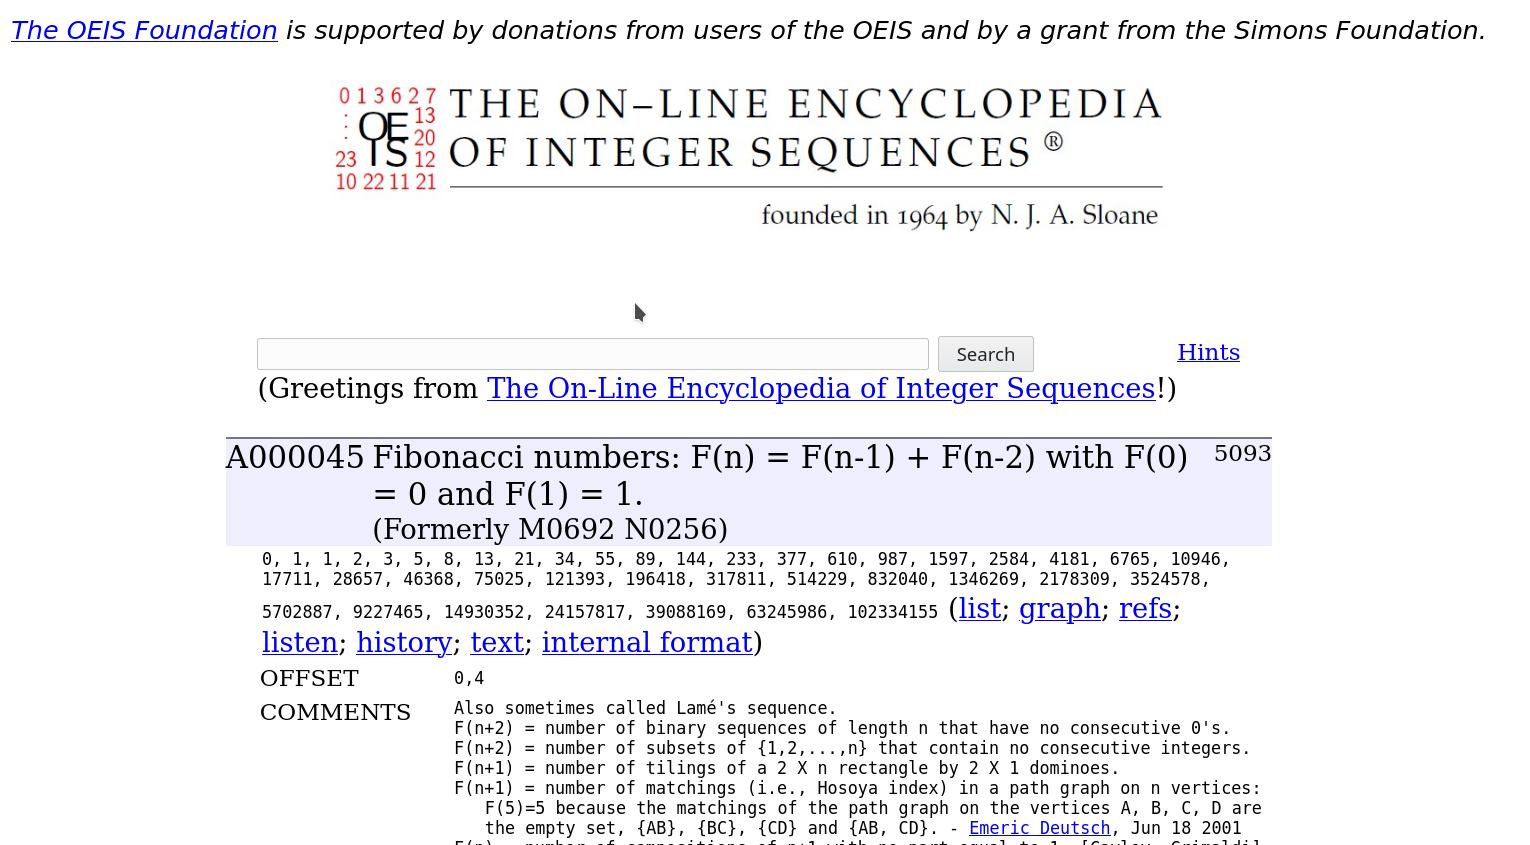
\includegraphics[width=13cm]{zoeis-pic.png}
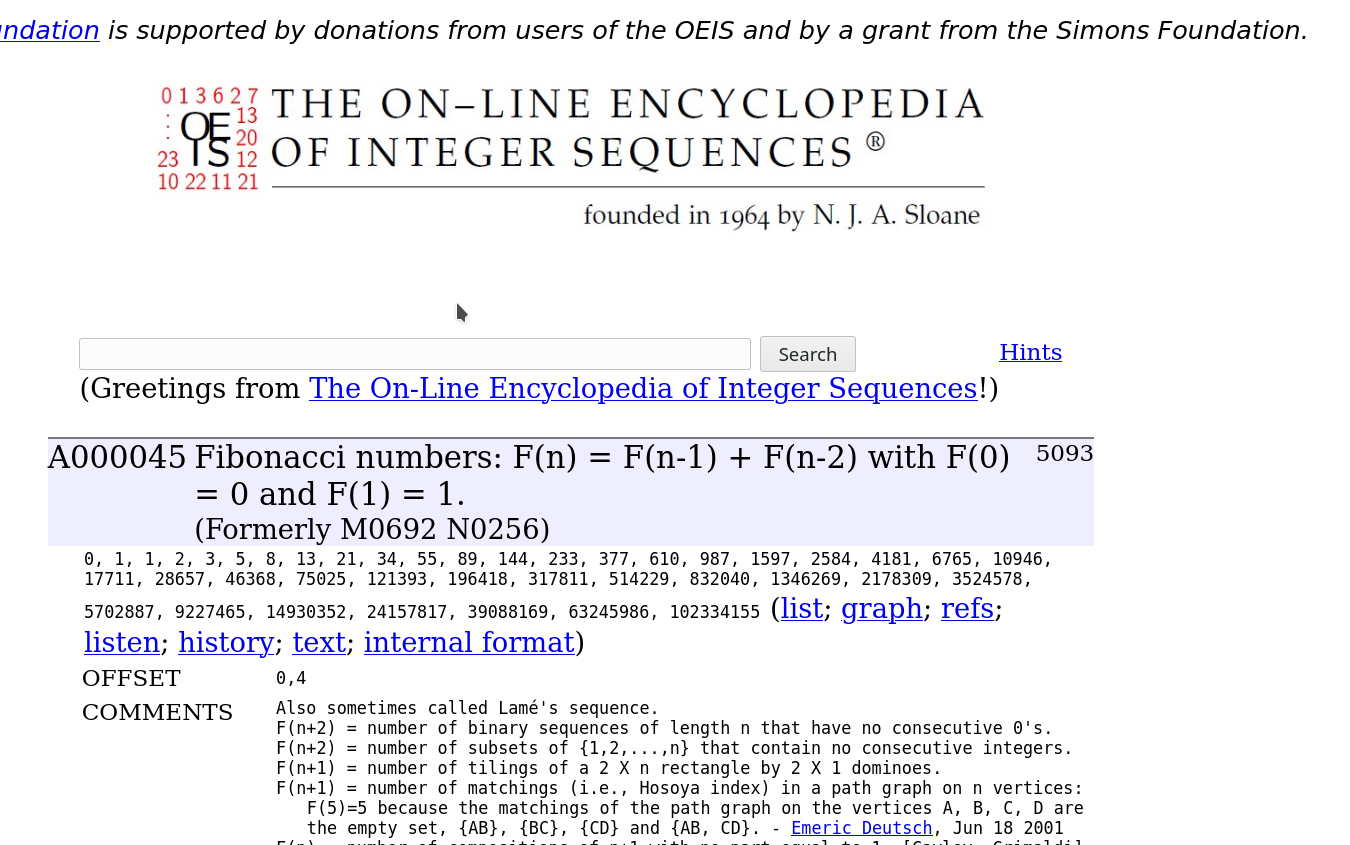
\includegraphics[width=13cm]{zoeis-c.png}
% Sedaj sledi še zaden del predstavitve, tj. celoštevilska zaporedja. 
\end{frame}


\begin{frame}
\begin{table}[h]
\centering
\begin{tabular}{cc}
\hline
ID & Name \\
\hline
A000009 
& Expansion of Product  \(\prod\limits_{m = 1}^\infty (1 + x^m)\) \\
A000040 & Prime numbers \\
A000045 & Fibonacci numbers \\
A000124 & Central polygonal numbers \\
A000219 & Number of planar partitions of $n$ \\
A000292 & Tetrahedral numbers \\
A000720 & Number of primes $\le n$ \\
A001045 & Jacobsthal sequence \\
A001097 & Twin primes \\
A001481 & Numbers that are the sum of 2 squares \\
A001615 & Dedekind psi function \\
A002572 & Number of partitions of 1 into n powers of 1/2 \\
A005230 & Stern's sequence \\
A027642 & Denominator of Bernoulli number $B_n$ \\
\hline
\end{tabular}
\caption{List of 14 sequences}
% \label{tab:zaporedja}
\end{table}
\end{frame}


 \begin{frame}{Dataset}

     \begin{itemize}
         \item Dataset is adjusted to the discovery of recursive equations of the form:
             % Podatkovna mno"zica je prilagojena odkrivanju rekurzivne ena"cbe: 
         $$ a_n = f(\vec{c}, n, a_{n-1}, ..., a_{n-49}) \enspace.  $$
         \item \[
 X :=
 \left[ 
 \begin{array}{ccccccccccccccccccccccccccccccccccccccccccccccccccc}
 1 & a_{0} & 0 & 0 & 0 & \cdots & 0 & 0 & 0 & a_{1} &  \\
 2 & a_{1} & a_{0} & 0 & 0 & \cdots & 0 & 0 & 0 & a_{2} &  \\
 3 & a_{2} & a_{1} & a_{0} & 0 & \cdots & 0 & 0 & 0 & a_{3} &  \\
 4 & a_{3} & a_{2} & a_{1} & a_{0} & \cdots & 0 & 0 & 0 & a_{4} &  \\
 5 & a_{4} & a_{3} & a_{2} & a_{1} & \cdots & 0 & 0 & 0 & a_{5} &  \\
 \vdots & & & & & \ddots  & & & & \vdots \\
 47 & a_{46} & a_{45} & a_{44} & a_{43} & \cdots & a_{0} & 0 & 0 & a_{47} &  \\
 48 & a_{47} & a_{46} & a_{45} & a_{44} & \cdots & a_{1} & a_{0} & 0 & a_{48} &  \\
 49 & a_{48} & a_{47} & a_{46} & a_{45} & \cdots & a_{2} & a_{1} & a_{0} & a_{49} &  \\
 \end{array}
 \right] \enspace.
 \]
     \end{itemize}
    
 \end{frame}


 \begin{frame}{Probabilistic grammar}

Probabilistic grammar in use:
 \scriptsize
 \begin{eqnarray*}
 E & \to & P / R\ [0.2]\ |\ P\ [0.8] \\
 P & \to & P + c * R\ [0.4]\ |\  c * R\ [0.3]\ |\ c\ [0.3] \\
 R & \to & M\ [0.60024]\ |\ sqrt\ (\ c * M\ )\ [0.133253]\ |\  \\
 & & exp\ (\ c * M \ )\ [0.133253]\ |\ 
 log\ (\ c * M \ )\ [0.133253]  \\
 M & \to & M * V\ [0.4]\ |\ V\ [0.6] \\
 V & \to & n\ [0.5]\  | \ 
 a_{n-1}\ [0.319672]  \ | \ 
 a_{n-2}\ [0.0965392]  \ | \ 
 a_{n-3}\ [0.0295993]  \ | \ \\ &&
 a_{n-4}\ [0.0095173]  \ | \  
 a_{n-5}\ [0.00349271]  \ | \ 
 a_{n-6}\ [0.00168534]  \ | \ \\ &&
 a_{n-7}\ [0.00114312]  \ | \ 
 a_{n-8}\ [0.00098046]  \ | \ 
 a_{n-9}\ [0.000931661]  \ | \ \\ &&
 a_{n-10}\ [0.000917021]\ | \ 
 a_{n-11}\ [0.000912629]\ | \ 
 a_{n-12}\ [0.000911311]\ | \ \\ &&
 a_{n-13}\ [0.000910916]\ | \ 
 a_{n-14}\ [0.000910798]\ | \ 
 a_{n-15}\ [0.000910762]\ | \ \\ &&
 a_{n-16}\ [0.000910751]\ | \ 
 a_{n-17}\ [0.000910748]\ | \ 
 a_{n-18}\ [0.000910747]\ | \  \\ &&
 a_{n-19}\ [0.000910747]\ | \ 
 a_{n-20}\ [0.000910747]\ | \   
 a_{n-21}\ [0.000910747]\ | \   \\
 % & & a_{n-21}\ [0.000910747]\ | \ a_{n-22}\ [0.000910747]\ | \ a_{n-23}\ [0.000910747]\ | \ a_{n-24}\ [0.000910747]\ | \   \\
 % & & a_{n-25}\ [0.000910747]\ | \ a_{n-26}\ [0.000910747]\ | \ a_{n-27}\ [0.000910747]\ | \ a_{n-28}\ [0.000910747]\ | \   \\
 % & & a_{n-29}\ [0.000910747]\ | \ a_{n-30}\ [0.000910747]\ | \ a_{n-31}\ [0.000910747]\ | \ a_{n-32}\ [0.000910747]\ | \   \\
 % & & a_{n-33}\ [0.000910747]\ | \ a_{n-34}\ [0.000910747]\ | \ a_{n-35}\ [0.000910747]\ | \ a_{n-36}\ [0.000910747]\ | \   \\
 % & & a_{n-37}\ [0.000910747]\ | \ a_{n-38}\ [0.000910747]\ | \ a_{n-39}\ [0.000910747]\ | \ a_{n-40}\ [0.000910747]\ | \   \\
 % & & a_{n-41}\ [0.000910747]\ | \ a_{n-42}\ [0.000910747]\ | \ a_{n-43}\ [0.000910747]\ | \ a_{n-44}\ [0.000910747]\ | \   \\
 % & & a_{n-45}\ [0.000910747]\ | \ a_{n-46}\ [0.000910747]\ | \ a_{n-47}\ [0.000910747]\ | \ a_{n-48}\ [0.000910747]\ | \   \\
 & & \vdots  \\
 & &  a_{n-49}\ [0.000910747]\ 
 \enspace.
 \end{eqnarray*}

 \end{frame}

  \begin{frame}{Probabilistic grammar}
      \begin{itemize}
          \item Expressions are of the form 
               $P/R$, where  $P$ is  polynomial and $R$ is monomial, where
              % Izrazi oblike $P/R$, where kjer je $P$ polinom in $R$ monom, pri "cemer
               in place of monomials we allow functions sqrt, exp and log.
              % v monomih lahko nastopajo funkcije sqrt, exp in log.
           \item Probabilities of rewriting rules of the form $(V \to a_{n-k})$  
          % \item Verjetnosti prepisovalnih pravil oblike $(V \to a_{n-k})$ 
                are descending in a way that their ratio is 
          % padajo na na"cin, da so verjetnosti v razmerju
          $r:r^2:r^3: \cdots :r^{49}$, where $r=\frac{3}{10}$.
      \end{itemize}
  \end{frame}

  \begin{frame}{Settings of the function 'test'}
      \begin{itemize}
          \item Equation error is defined in the same way as on first slides.
          % \item Napaka ena"cbe definirana enako kot na za"cetnih prosojnicah.
          \item Optimization algorithm of differential evolution.
          % \item Optimizacijski algoritem diferencialne evolucije.
          \item Interval for optimization was set to $[-4, 4]$.
          % \item Interval, na katerem je potekala optimizacija konstant je $[-4, 4]$.
      \end{itemize}
  \end{frame}


  \begin{frame}{Number of generated equations}
  % \begin{frame}{"Stevilo tvorjenih ena"cb}
      \begin{itemize}
          \item $N = 100$
      \end{itemize}
  \end{frame}


\begin{frame}{Results}
    \scriptsize
% \begin{table}[H]
% \centering
$$    \begin{array}{cl}
\hline
    % \text{kraj"se ime } & 
    \text{Sequence ID} & \text{Equations discovered} \\
\hline
    % \text{Razvoj $\prod\limits_{m = 1}^\infty (1 + x^m)$}  & 
    A000009 
& \text{none} \\
    % \text{Pra"stevila} & 
    A000040 &  \text{none}   \\
\hline
    % \multirow{4}{*}{\text{Fibonaccijevo zaporedje}} & 
    \multirow{4}{*}{A000045} & a_n = 0.4472*exp(0.4812*n)  \\
    & a_n = 0.9886*a_{n-1} + 1.018*a_{n-2} \\
    & a_n = 2.618*a_{n-2} + 0.03653 \\
    & a_n = 1.591*a_{n-1} + 0.07085*a_{n-3} + 0.01706   \\
\hline
    % \multirow{2}{*}{\text{Leni natakar}} & 
    \multirow{2}{*}{A000124} & a_n =   0.992*a_{n-1} + 0.007*a_{n-2} + 1.007*n - 0.006 \\
    & a_n =   2.081*a_{n-1} - 1.083*a_{n-2} \\
\hline
    % \text{Ravninske raz"clenitve}  &
    A000219 &  \text{none} \\
\hline
    % \text{Tetraedri"cna "stevila} & 
    A000292 & a_n =  1.999*a_{n-1} - 0.999*a_{n-2} + 1.000*n -  0.000 \\
\hline
    % \text{pra"stevil manj"sa od $n$} &
    A000720 & \text{none} \\
\hline
    % \multirow{2}{*}{\text{Jacobsthalovo zaporedje}} &  
    \multirow{2}{*}{A001045} & a_n =   1.000*a_{n-1} + 1.998*a_{n-2} \\
    & a_n =   2.956*a_{n-1} - 3.824*a_{n-3} - 0.029        \\
\hline
    % \text{Pra"stevilski dvoj"cki} & 
    A001097 & \text{none} \\
    % \text{Vsote dveh kvadratov} & 
    A001481 & \text{none} \\
    % \text{Dedekindova funkcija psi} & 
    A001615 & \text{none} \\
    % \text{raz"clenitve 1 na potence $\frac{1}{2}$} & 
    A002572 & \text{none} \\
    % \text{Sternovo zaporedje} & 
    A005230 & \text{none} \\
    % \text{Imenovalec Bernoullijevega "stevila } & 
    A027642 & \text{none} \\
\hline
\end{array}$$

%!!! Naslovi tabel naj bodo daljši in samozadostni: bralec bi moral le iz naslova razumeti vsebino tabele!
% \caption{Povzetek rezultatov rekonstrukcije enačb za štirinajst izbranih zaporedij iz OEIS.}
% \label{tab:povzetek rezultatov}
% \end{table}
\end{frame}


%% \begin{frame}
%% \begin{itemize}
%% % [<+->]
%%     \item Poganjal nad celoštevilskimi zaporedji.
%% % Algoritem za odkrivanje enačb z verjetnostnimi gramatikami sem poganjal na podatkih sestavljenih iz celoštevilskih zaporedij.
%%     \item Pridobil na oeis.org
%% % Celoštevilska zaporedja sem dobil na spletni strani oeis.org, tj. spletna enciklopedija celoštevolskih zaporedij. (Ki je bila prikazana na prej"snji prosolnici.)
%%     \item Na voljo ve"c kot 340 000 zaporedij.
%%     \item Poleg prvih "clenov zaporedja tudi opis, klju"cne besede, formule, reference, ...
%% \end{itemize}
%% \end{frame}

%% \begin{frame}
%% \begin{itemize}
%% % {Izbor zaporedij}
%% % [<+->]
%%     \item Izbor 108 zaporedij.
%% % Jaz sem svoj izbor zaporedij omejil na 108 zaporedij.
%%     \item Vklju"citev pomemebnih zaporedij \\
%%     344.012 $\to$ 178 zaporedij \\
%%     keyword:core 
%%     % format
%% %  \url{https://oeis.org/eishelp2.html#RK}
%% % Najprej sem se omejili na 178 zaporedij tako, da sem izbral samo zaporedja s klju"cno besedo core, 
%% % 344.012 $\to$ 178 zaporedij \\
%%     \item Izklju"citev trivialnih zaporedij
%%     (1,1,1,...), (0,0,0,...), (1,2,3,...), (-1,-2,-3,...), ... \\
%%     178 $\to$ 171 zaporedij \\ 
%%     keyword:nice 
%% % Nato smo se izmed teh dodatno omejili na tiste s kljuˇcno
%% % besedo nice in se s tem izognili trivialnim zaporedjem, kot so npr. konstan-
%% % tno zaporedje samih enic (1,1,1,...), niˇcel (0,0,0,...), zaporedje naravnih ˇstevil
%% % (1,2,3,...), negativnih ˇstevil (-1,-2,-3,...), ipd.
%% % Tako sem odstranil 7 zaporedij.
%%     \item Izklju"citev zaporedij z manj kot 50 "cleni \\
%%     171 $\to$ 163 zaporedij \\ 
%%     -keyword:more \\
%% % Potem sem od preostalih odstranil 8 zaporedij, ki imajo manj kot 50
%% % znanih ˇclenov zaporedja. Ta so nosila ključno besedo more ali hard. Na ta način sem prišel na 163 zaporedij. 
%% % \item odstrantev zaporedja $\mersenne$ znotraj keyword:hard $\dots$ 164 $\to$ 163 zaporedij
%%     \item Izklju"citev zaporedij s "cleni ve"cjimi od $10^{16}$ \\
%%     163 $\to$ 108 zaporedij \\ 
%%     % Nato sem odstranil še vsa zaporedija, ki imajo izmed prvih 50 ˇclenov kakˇsen ˇclen z
%%     % absolutno vrednostjo veˇcjo od 10^6 in tako prišel do množice 108-ih zaporedij. 
%%     \pause
%%     \item \textcolor{red}{50 "clenov na zaporedje}
%% % Od vskaega zaporedja sem vzel smao prvih 50 členov zaporedja
%% \end{itemize}
%% \end{frame}


%% \begin{frame}{Celo"stevilskih zaporedija: do sedaj}
%% % Sedaj lahko povem kaj so bili vhodni podatki v mojem primeru
%% % celo"stevilskih zaporedij.
%% \begin{itemize}
%% % [<+->]
%% % Do sedaj sem odkrival enačbe znotraj celoštevilskih zaporedij na naslednji način:
%%     \only<1-1>{\item Pognal za vsako zaporedje posebej.}
%% % Treba je povdariti, da sem pognal za vsako zaporedje posebej. 
%%     \item Odkrival ve"c razli"cnih oblik ena"cb:
%%     \begin{itemize}
%%         \item v zaprti obliki:  \(a_n =f(n)\)
%%         %  n-ti "clen zaporedja je odvisen samo od n.
%%         \ \ \ \ \ \ \ \ \ \
%%             \( \left[ \begin{array}{cc}
%%                 1 & a_1 \\
%%                 2 & a_2 \\
%%             \vdots & \vdots \\
%%                 50 & a_{50} 
%%             \end{array} \right] \)
%%         \pause
        
%%         \item rekurzivne rede 4:
%%         \( a_n = f(n, a_{n-1} , a_{n-2}, a_{n-3} .. , a_{n-4})\) \ \ \ \
%%         %  n-ti "clen zaporedja je odvisen prej"snjih m
%%             \hspace{4cm} \datasetn{4}
        
%%         \item rekurzivne rede 4, kjer n ne nastopa:  
%%         \( a_n = f(a_{n-1} , a_{n-2}, a_{n-3} .. , a_{n-4})\) \ \ \ \
%%             \dataset{4}
%%             % \pause
%%     \end{itemize}
%%     % \item Vhodni podatki prirejeni vrsti "zeljenih ena"cb.
%% % Za vsako zaporedje sem izdelal prirejeno podatkovno množico za algoritem za odkrivanje enačb, glede na to, kakšen tip enačbe sem odkrival.
%% \end{itemize}
%% \end{frame}



%% % \begin{frame}{Konstrukcija vhodnih podatkov}

%% % % Podatkovno množico sem zgradil tako:
%% % \begin{itemize}
%% %     % [<+->]
%% %     \item Stolpec s prvimi 50 členi zaporedja.
%% %     % Začel sem s prvim stolpcem s prvimi 50 členi zaporedja. 
%% %     \item Dodal m (red rekurzije) zamaknjenih stolpcev. \\
%% %     % Nato sem glede na red m dodal m stolpcev, kjer sem i-ti stolpec zamaknil za 1 navzgor, (tj. 
%% %     % odstranil sem  prvih i členov in i+prvega dal na prvo mesto ter na koncu matriko na dnu odrezal, da ni vsebovala praznih členov.)
%% %     Dobil \( (n-m) \times (m+1) \) matriko.
%% %     % Tako sem dobil n-m x m+1 matriko.
%% %     \item V primeru ena"cb odvisnih od n dodal stolpec naravnih "stevil.
%% % % Nato sem v primeru iskanja direktne enačbe dodal še stolpec privih 50 naravnih števil. 
%% % \end{itemize}
%% % \end{frame}

    
%% % \begin{frame}{Podrobneje}
%% %     \begin{itemize}
%% %     % % [<+->]
%% %         \item Za isto zaporedje algoritem pognal 5-krat.
%% %     % % Vhodni podatki so bili seveda vsaki"c razli"cni, razlika pa v
%% %     % % tem, kak"sne ena"cbe sem odkrival.
%% %         \item Odkrival naslednje tipe ena"cb:
%% %         \begin{itemize}
%% %             % \item rekurzivne reda 2:
%% %             %     \datatwo{2}
%% %             \item rekurzivne reda 4:
%% %                 \dataset{4}
%% %         \end{itemize}
%% %     \end{itemize}
%% % \end{frame}

%% % \begin{frame}
%% %     \begin{itemize}
%% %         \item odvisne od n in rekurzivne reda 0: \\
%% %             \( \left[ \begin{array}{c|c}
%% %                 1 & a_1 \\
%% %                 2 & a_2 \\
%% %             \vdots & \vdots \\
%% %                 50-m & a_{50-m} 
%% %             \end{array} \right] \)
%% %         % \item odvisne od n in rekurzivne reda 2:
%% %         %     \datatwon{2}
%% %         \item odvisne od n in rekurzivne reda 4:
%% %             \datasetn{4}
%% %     \end{itemize}
%% % \end{frame}

%% \begin{frame}
%% % {Uporabljena gramatika}
%% Predloga gramatike vsaki"c polinomska. \\
%% \begin{block}{Predloga polinomske gramatike}
%%     S $\to$ S '+' R [0.4] \\
%%     S $\to$ R [0.6] \\
%%     R $\to$ T [0.6] \\
%%     R $\to$ 'C' '*' F '(' T ')' [0.4] \\
%%     T $\to$ T '*' V [0.4] \\
%%     T $\to$ 'C' [0.6] \\
%%     F $\to$ 'exp' [1.0] \\
%%     V $\to$ 'n' [0.333] \\
%%     V $\to$ 'an\_4' [0.333] \\
%%     V $\to$ 'an\_3' [0.333] \\
%%     V $\to$ 'an\_2' [0.333] \\
%%     V $\to$ 'an\_1' [0.333] \\
%% \end{block}

%% kjer se pravila z nekon"cne simbole V spremenijo
%% glede na obliko ena"cb.
%% % Izbral sem polinomsko gramatiko, ki izgleda takole:

%% \end{frame}


%% \begin{frame}{Dodatne nastavitve algoritma}
%%     \begin{itemize}
%%         \item Število generiranj struktur izrazov: 100
%%         \item Interval optimizacije konstant: (-5, 5)
%%         % ali (-10, 10)
%%     %   - v primeru reda 0 (in privzete direktne enačbe) sem doovljeal poljubne konstante na določenem intervalu (od -10? Do 10?)
%%         \item Napaka modela: Predhodna zaokro"zitev konstant v primeru rekurzivnih oblik ena"cb v izogib racionalnih "clenov.
%%     %   - v primeru reda 1 ali več pa sem se omejil na celoštevilske konstante znotraj izraza. To sem dosegel tako, da sem spremenil napako modela, ki na mestu konstant vsebuje zaokrožene vrednosti konstant.
%%     \end{itemize}
%% \end{frame}


%% % \begin{frame}{Rezultati}
%% % % Čeprav sem algoritem pognal za vseh 108 zaporedij, vseh rezultatov nisem še uspel analizirati. Sem pa bolj podrobneje analiziral rezultate za Fibonaccijevo zaporedje. Algoritem je uspešno odkril tako rekurzivno enačbo a_n = a_n-1 in a_n-2 in direktno enačbo v obliki an = [c0 * exp( n*c1)] , kar mogoče zveni bolj znano kot 
%% % % a_n = [ c1*phi ** n] = phi *n - psi**n .
%% %     \begin{itemize}
%% %         \item Vsi rezultati "se niso analizirani.
%% %         \item Rezultati za Fibonaccijevo zaporedje so analizirani.
%% %         \begin{itemize}
%% %             \item Odkrita rekurzivna ena"cba: 
%% %                 \( a_n = a_{n-1} + a_{n-2} \)
%% %             \item Odkrita ena"cba v zaprti obliki: 
%% %                 \( a_n = [ 0.447213 \cdot e^{ n \cdot 0.481211} ] \)  \\
%% %                 \pause
%% %                 \( = [ \frac{1}{\sqrt{5}} \cdot e^{ n \cdot \ln(\varphi)} ]  \) \\
%% %                 % \pause
%% %                 \(  = [\frac{\varphi^n}{\sqrt{5}}]
%% %                     = \frac{\varphi^n -\psi^n}{\sqrt{5}} \) \\
%% %                 kjer [ \ \ ] predstavlja zaokro"zevanje, 
%% %                 \( \varphi = \frac{1+\sqrt{5}}{2} \) zlati rez in
%% %                 \( \psi = \frac{1-\sqrt{5}}{2} \).
%% %                 \pause
%% %             \item Algoritem je izpisal:
%% %         \end{itemize}
%% %     \end{itemize}
%% %             \texttt{model: 0.447213595444298*exp(0.481211825062448*n); \\
%% % error: 0.006827339418724309
%% % }                
%% % \end{frame}

%% \begin{frame}{Rezultati}
%% % Čeprav sem algoritem pognal za vseh 108 zaporedij, vseh rezultatov nisem še uspel analizirati. Sem pa bolj podrobneje analiziral rezultate za Fibonaccijevo zaporedje. Algoritem je uspešno odkril tako rekurzivno enačbo a_n = a_n-1 in a_n-2 in direktno enačbo v obliki an = [c0 * exp( n*c1)] , kar mogoče zveni bolj znano kot 
%% % a_n = [ c1*phi ** n] = phi *n - psi**n .
%%     \begin{itemize}
%%         % \item \[ \phi = 1.618033988749895 \] 
%%         % \item \[ \frac{1}{\sqrt{5}} = 0.4472135954999579 \] 
%%         % \item \[ \ln(phi) = 0.48121182505960347 \]
%% %         >> 1/(5**(1/2))
%% % sqrt(5) = 2.23606797749979
%% % phi = 1.618033988749895
%% % 1/sqrt(5) = 0.4472135954999579
%% % ln(phi) = 0.48121182505960347

%%         \only<1-2>{\item Vsi rezultati "se niso analizirani.}
%%         \item Rezultati za Fibonaccijevo zaporedje so analizirani.
%%         \begin{itemize}
%%             \only<1-2>{
%%             \item Odkrita rekurzivna ena"cba: 
%%                 \( a_n = a_{n-1} + a_{n-2} \)}
%%             \item Odkrita ena"cba v zaprti obliki: 
%%                 \( a_n = 0.447213595444298 \cdot e^{ n \cdot 0.481211825062448} \)  \\
%%                 \pause
%%         \end{itemize}
%%     \end{itemize}
%%     \only<1-2>{
%%     Algoritem je izpisal: \\
%%         \texttt{model: 0.447213595444298*exp(0.481211825062448*n); \\
%%     %   4472135954|999579   0.4812118250|5960347
%%     error: 0.006827339418724309} \\}
%%     \pause
%%     Smiselno, saj: \\
%%     \( a_n = \frac{\varphi^n -\psi^n}{\sqrt{5}} \)
%%     \( = [\frac{\varphi^n}{\sqrt{5}}] \)
%%     \( = [ \frac{1}{\sqrt{5}} \cdot e^{ n \cdot \ln(\varphi)} ]  \) \\
%%         % = \frac{\varphi^n -\psi^n}{\sqrt{5}} \) \\
%%     kjer [ \ \ ] predstavlja zaokro"zevanje, 
%%     \( \varphi = \frac{1+\sqrt{5}}{2} \) zlati rez in
%%     \( \psi = \frac{1-\sqrt{5}}{2} \).
%%     \pause \\
%%     Primerjava: 
%%     \[\begin{array}{lll}
%%          & \frac{1}{\sqrt{5}} & \ln(\varphi) \\
%%          \hline
%%         \text{algoritem} & 0.447213595444298 & 0.481211825062448  \\
%%          \text{dejansko} & 0.447213595499957 & 0.481211825059603 
%%                 \end{array}\]
        
%% \end{frame}

%% \begin{frame}{Zlati rez}
%% % Izpisal je tudi nekaj na kar nisem pomislil pred poganjanjem zaporedja in sicer:
%%     Algoritem je izpisal: \\
%% \texttt{model: 2.61803398874827*an\_2         ; error: 
%% 0.03370982707452994 \\
%% model: 1.61803398874905*an\_1         ; error: 0.012876264161607837
%% } \\
%% \vspace{0.4cm}
%% Druga številka \texttt{1.618...} je zlati rez in 
%% prva \texttt{2.618...} njegov kvadrat.  \\
%% Zlati red je namreč ravno pribli"zek razmerja 
%%  \( \varphi \approx \frac{a_n}{a_{n-1}} \), 
%%  kar pomeni \( a_n \approx \varphi \cdot a_{n-1} \)
%% in posledično \( a_n \approx \varphi \cdot ( \varphi  a_{n-1}) = \varphi^2 \cdot a_{n-2} \).
%% \pause
%%     Primerjava: 
%%             \[\begin{array}{lll}
%%              & \varphi & \varphi^2 \\
%%              \hline
%%     \text{algoritem} & 1.61803398874827 & 2.61803398874827  \\
%%      \text{dejansko} &  1.61803398874989 &  2.61803398874989
%%             \end{array}\]
%% \end{frame}


%% % \begin{frame}{Kaj me "se "caka}
%% % % Kar bom še naredil:
%% % %  Poskušal bom odkrivati razmerja med zaporedji.
%% %     \begin{itemize}
%% %         \item Ena"cbe povezovanja med zaporedji.
%% %         % \item Hierarhi"cno rojenje glede na kovarianco med zaporedji.
%% % % To neravam narediti tako, da bom najprej s pomočjo hierarhičnega rojenja glede na kovarianco razvrstil podobna zaporedja v skupine. 
%% %         % \item Znotraj skupine: zaporedja kot stolpci
%% % % Zaporedja znotraj ene skupine bom  sestavil v podatkovno množico, tako, da bom stolpce zložil enega poleg drugega v matriko ter nato s pomočjo algoritma za odkrivanje enačb poskušal odkriti enačbo, ki jih povezuje.
%% %     \end{itemize}
%% % \end{frame}



%% % \begin{frame}{Viri in literatura}
%% % \begin{itemize}
%% %     \item J. Brence, \textit{From Deterministic to Probabilistic Approaches in Automated Modeling}, Seminar 1, Ljubljana, 2020.
%% %     \item Z. Chi,
%% %     \textit{Statistical properties of probabilistic context-free grammars}, 
%% %     Computational Linguistics, 
%% %     \textbf{25}(1), (1999), 131--160 
%% %     % https://www.semanticscholar.org/paper/Statistical-Properties-of-Probabilistic-Grammars-Chi/2acaf3499642c68d4f905209ec0dd508c0648696
%% %     \item S. Geman in M. Johnson. 
%% %     \textit{Probabilistic grammars and their applications}, International Encyclopedia of the Social \& Behavioral Sciences, Oxford, Pergamon 2001, 12075--12082.
%% % %     % https://www.sciencedirect.com/referencework/9780080430768/international-encyclopedia-of-the-social-and-behavioral-sciences
%% % %     % https://www.dam.brown.edu/people/geman/Homepage/Computational%20linguistics/Computational%20linguistics.htm
%% % %     % https://doi.org/10.1016/B0-08-043076-7/00489-7
%% %     \item T.E. Harris, \textit{The Theory of Branching Processes}, 
%% %     Berlin, Springer-Verlag Berlin Heidelberg 1963, str. 34.
%% %     \item M.I. Miller, \textit{Entropies and combinatorics of random branching processes and context-free languages},
%% %     IEEE Transactions on Information Theory, 
%% %     \textbf{38}(4), (1992), 1292--1295 
%% %     % https://ieeexplore.ieee.org/document/144710
%% %     \item L. Todorovski,
%% %     \textit{Declarative Bias of Equation Discovery}, 
%% %     Magisterska naloga,
%% %     Ljubljana, 1998.
%% %     % https://www.semanticscholar.org/paper/Declarative-Bias-in-Equation-Discovery-Todorovski/e3c42c7055ba7ec73cff445c779096c1211cb3b9
%% % \end{itemize}
%% % \end{frame}




\begin{frame}{Sources and literature}
% \begin{frame}{Viri in literatura}
\begin{itemize}
    \item J. Blazej, \textit{Procesi razvejanja}, diplomsko delo, Fakulteta za matematiko in fiziko, Univerza v Ljubljani, 2016.
    \item J. Brence, \textit{From Deterministic to Probabilistic Approaches in Automated Modeling}, Ljubljana, 2020.
    \item J. Brence, L. Todorovski in S. Džeroski, \textit{Probabilistic grammars for equation discovery}, Knowledge-Based Systems \textbf{224} (2021), doi: 10.1016/j.knosys.2021.  107077.
    \item Z. Chi, \textit{Statistical properties of probabilistic context-free grammars}, Computational Linguistics \textbf{25}(1) (1999) 131–160, doi: 10.5555/973215.973219.
    \item M. Collins, \textit{Probabilistic Context-Free Grammars (PCFGs)}, [ogled 9. 6. 2021], dostopno na \url{www.cs.columbia.edu/~mcollins/courses/nlp2011/notes/pcfgs.pdf}.
\end{itemize}
\end{frame}


\begin{frame}
\begin{itemize}
    \item  T. Csernica, \textit{Extinction in single and multi-type branching processes}, [ogled 9. 6.  2021], dostopno na \url{http://math.uchicago.edu/~may/REU2015/REUPapers/ Csernica.pdf}.
    \item T. Harris, \textit{The Theory of Branching Processes}, Grundlehren der mathematischen Wissenschaften \textbf{119}, Springer-Verlag Berlin Heidelberg, Berlin, 1963.
    \item S. G. in M. Johnson, \textit{Probabilistic grammars and their applications}, International Encyclopedia of the Social \& Behavioral Sciences \textbf{158}, Pergamon, Oxford, 2001.
    \item M. Jiřina, \textit{A simplified proof of the sevastyanov theorem on branching processes}, Annales de l’I.H.P. Probabilités et statistiques \textbf{6}(1) (1970) 1–7.
    \item M. Miller, \textit{Entropies and combinatorics of random branching processes and context-free languages}, IEEE Transactions on Information Theory \textbf{38}(4) (1992) 1292–1310, doi: 10.1109/18.144710.

\end{itemize}
\end{frame}

\begin{frame}
\begin{itemize}
    \item C. J. Mode, \textit{Multitype Branching Processes: Theory and Applications}, Modern analytic and computational methods in science and mathematics, American Elsevier Publishing Company, New York, 1971.
    \item M. Schmidt in H. Lipson, \textit{Distilling free-form natural laws from experimental data}, Science (New York, N.Y.) \textbf{324} (2009) 81–85, doi: 10.1126/science.  1165893.
    \item N. J. A. Sloane, \textit{The On-Line Encyclopedia of Integer Sequences}, [ogled 1. 6.  2021], dostopno na \url{https://oeis.org}.
    \item R. Storn in K. Price, \textit{Differential evolution – a simple and efficient heuristic for global optimization over continuous spaces}, Journal of Global Optimization \textbf{11} (1997) 341–359, doi: 10.1023/A:1008202821328.
    \item L. Todorovski, \textit{Declarative Bias of Equation Discovery}, magistsko delo, Fakulteta za računalništvo in informatiko, Univerza v Ljubljani, 1998.
\end{itemize}
\end{frame}

\begin{frame}
\begin{itemize}
    \item L. Todorovski, \textit{Odkrivanje enačb in predznanje}, Ljubljana, 2021, prosojnice pri predmetu Napredno strojno učenje, [ogled 14. 7. 2021], dostopno na \url{http://kt.ijs.si/~ljupco/lectures/nsu/11-ed-knowledge.pdf}.
    \item L. Todorovski, \textit{Uvod v odkrivanje enačb in simbolno regresijo}, Ljubljana, 2021, prosojnice pri predmetu Napredno strojno učenje, [ogled 14. 7. 2021], dostopno na \url{http://kt.ijs.si/~ljupco/lectures/nsu/10-ed-intro.pdf}.
\item L. Todorovski in S. Džeroski, \textit{Declarative bias in equation discovery}, v: ICML ’97: Proceedings of the Fourteenth International Conference on Machine Learning, Morgan Kaufmann Publishers, San Francisco, ZDA, 1997, str. 376–384, doi: 10.5555/645526.657279.

\end{itemize}
\end{frame}
% \begin{frame}
% \begin{itemize}

\begin{frame}
\end{frame}
\begin{frame}
\end{frame}
\begin{frame}
\end{frame}
\begin{frame}
\end{frame}



\begin{frame}
    \label{Seva}
    \sevast

\begin{block}{Theorem: Sevast'yanov}

    Let $\rho$ be spectral radius of 
    matrix $M$ of first moments of multitype branching process.
    Then extinction probability vector equals to $\mathbf{q = 1}$
    if and only if:
    
(a) \( \rho \le 1 \) and \\
(b) it has no \textbf{final classes}.

\end{block}

 \hyperlink{Thm}{\beamergotobutton{-}}

\end{frame}


\end{document}

% % \begin{frame}{Algoritem za odkrivanje ena"cb}
% % \begin{itemize}
% % [<+->]
% %     \item dsa
% % \end{itemize}
% % \end{frame}
